% Options for packages loaded elsewhere
\PassOptionsToPackage{unicode}{hyperref}
\PassOptionsToPackage{hyphens}{url}
\PassOptionsToPackage{dvipsnames,svgnames,x11names}{xcolor}
%
\documentclass[
  12pt,
  letterpaper,
  DIV=11,
  numbers=noendperiod]{scrartcl}

\usepackage{amsmath,amssymb}
\usepackage{lmodern}
\usepackage{iftex}
\ifPDFTeX
  \usepackage[T1]{fontenc}
  \usepackage[utf8]{inputenc}
  \usepackage{textcomp} % provide euro and other symbols
\else % if luatex or xetex
  \usepackage{unicode-math}
  \defaultfontfeatures{Scale=MatchLowercase}
  \defaultfontfeatures[\rmfamily]{Ligatures=TeX,Scale=1}
\fi
% Use upquote if available, for straight quotes in verbatim environments
\IfFileExists{upquote.sty}{\usepackage{upquote}}{}
\IfFileExists{microtype.sty}{% use microtype if available
  \usepackage[]{microtype}
  \UseMicrotypeSet[protrusion]{basicmath} % disable protrusion for tt fonts
}{}
\makeatletter
\@ifundefined{KOMAClassName}{% if non-KOMA class
  \IfFileExists{parskip.sty}{%
    \usepackage{parskip}
  }{% else
    \setlength{\parindent}{0pt}
    \setlength{\parskip}{6pt plus 2pt minus 1pt}}
}{% if KOMA class
  \KOMAoptions{parskip=half}}
\makeatother
\usepackage{xcolor}
\usepackage[margin=1in]{geometry}
\setlength{\emergencystretch}{3em} % prevent overfull lines
\setcounter{secnumdepth}{-\maxdimen} % remove section numbering
% Make \paragraph and \subparagraph free-standing
\ifx\paragraph\undefined\else
  \let\oldparagraph\paragraph
  \renewcommand{\paragraph}[1]{\oldparagraph{#1}\mbox{}}
\fi
\ifx\subparagraph\undefined\else
  \let\oldsubparagraph\subparagraph
  \renewcommand{\subparagraph}[1]{\oldsubparagraph{#1}\mbox{}}
\fi


\providecommand{\tightlist}{%
  \setlength{\itemsep}{0pt}\setlength{\parskip}{0pt}}\usepackage{longtable,booktabs,array}
\usepackage{calc} % for calculating minipage widths
% Correct order of tables after \paragraph or \subparagraph
\usepackage{etoolbox}
\makeatletter
\patchcmd\longtable{\par}{\if@noskipsec\mbox{}\fi\par}{}{}
\makeatother
% Allow footnotes in longtable head/foot
\IfFileExists{footnotehyper.sty}{\usepackage{footnotehyper}}{\usepackage{footnote}}
\makesavenoteenv{longtable}
\usepackage{graphicx}
\makeatletter
\def\maxwidth{\ifdim\Gin@nat@width>\linewidth\linewidth\else\Gin@nat@width\fi}
\def\maxheight{\ifdim\Gin@nat@height>\textheight\textheight\else\Gin@nat@height\fi}
\makeatother
% Scale images if necessary, so that they will not overflow the page
% margins by default, and it is still possible to overwrite the defaults
% using explicit options in \includegraphics[width, height, ...]{}
\setkeys{Gin}{width=\maxwidth,height=\maxheight,keepaspectratio}
% Set default figure placement to htbp
\makeatletter
\def\fps@figure{htbp}
\makeatother
\newlength{\cslhangindent}
\setlength{\cslhangindent}{1.5em}
\newlength{\csllabelwidth}
\setlength{\csllabelwidth}{3em}
\newlength{\cslentryspacingunit} % times entry-spacing
\setlength{\cslentryspacingunit}{\parskip}
\newenvironment{CSLReferences}[2] % #1 hanging-ident, #2 entry spacing
 {% don't indent paragraphs
  \setlength{\parindent}{0pt}
  % turn on hanging indent if param 1 is 1
  \ifodd #1
  \let\oldpar\par
  \def\par{\hangindent=\cslhangindent\oldpar}
  \fi
  % set entry spacing
  \setlength{\parskip}{#2\cslentryspacingunit}
 }%
 {}
\usepackage{calc}
\newcommand{\CSLBlock}[1]{#1\hfill\break}
\newcommand{\CSLLeftMargin}[1]{\parbox[t]{\csllabelwidth}{#1}}
\newcommand{\CSLRightInline}[1]{\parbox[t]{\linewidth - \csllabelwidth}{#1}\break}
\newcommand{\CSLIndent}[1]{\hspace{\cslhangindent}#1}

\usepackage{booktabs}
\usepackage{longtable}
\usepackage{array}
\usepackage{multirow}
\usepackage{wrapfig}
\usepackage{float}
\usepackage{colortbl}
\usepackage{pdflscape}
\usepackage{tabu}
\usepackage{threeparttable}
\usepackage{threeparttablex}
\usepackage[normalem]{ulem}
\usepackage{makecell}
\usepackage{xcolor}
\usepackage[default]{sourcesanspro}
\usepackage{sourcecodepro}
\usepackage{lineno}
\linenumbers
\linespread{1.2}
\KOMAoption{captions}{tableheading}
\makeatletter
\makeatother
\makeatletter
\makeatother
\makeatletter
\@ifpackageloaded{caption}{}{\usepackage{caption}}
\AtBeginDocument{%
\ifdefined\contentsname
  \renewcommand*\contentsname{Table of contents}
\else
  \newcommand\contentsname{Table of contents}
\fi
\ifdefined\listfigurename
  \renewcommand*\listfigurename{List of Figures}
\else
  \newcommand\listfigurename{List of Figures}
\fi
\ifdefined\listtablename
  \renewcommand*\listtablename{List of Tables}
\else
  \newcommand\listtablename{List of Tables}
\fi
\ifdefined\figurename
  \renewcommand*\figurename{Fig.}
\else
  \newcommand\figurename{Fig.}
\fi
\ifdefined\tablename
  \renewcommand*\tablename{Table}
\else
  \newcommand\tablename{Table}
\fi
}
\@ifpackageloaded{float}{}{\usepackage{float}}
\floatstyle{ruled}
\@ifundefined{c@chapter}{\newfloat{codelisting}{h}{lop}}{\newfloat{codelisting}{h}{lop}[chapter]}
\floatname{codelisting}{Listing}
\newcommand*\listoflistings{\listof{codelisting}{List of Listings}}
\makeatother
\makeatletter
\@ifpackageloaded{caption}{}{\usepackage{caption}}
\@ifpackageloaded{subcaption}{}{\usepackage{subcaption}}
\makeatother
\makeatletter
\@ifpackageloaded{tcolorbox}{}{\usepackage[many]{tcolorbox}}
\makeatother
\makeatletter
\@ifundefined{shadecolor}{\definecolor{shadecolor}{rgb}{.97, .97, .97}}
\makeatother
\makeatletter
\makeatother
\ifLuaTeX
  \usepackage{selnolig}  % disable illegal ligatures
\fi
\IfFileExists{bookmark.sty}{\usepackage{bookmark}}{\usepackage{hyperref}}
\IfFileExists{xurl.sty}{\usepackage{xurl}}{} % add URL line breaks if available
\urlstyle{same} % disable monospaced font for URLs
\hypersetup{
  colorlinks=true,
  linkcolor={blue},
  filecolor={Maroon},
  citecolor={Blue},
  urlcolor={Blue},
  pdfcreator={LaTeX via pandoc}}

\author{}
\date{}

\begin{document}
\ifdefined\Shaded\renewenvironment{Shaded}{\begin{tcolorbox}[sharp corners, boxrule=0pt, borderline west={3pt}{0pt}{shadecolor}, interior hidden, frame hidden, breakable, enhanced]}{\end{tcolorbox}}\fi

\textbf{Running title}: Metabolic and structural leaf mass

\textbf{Decomposing leaf mass into metabolic and structural components
explains divergent patterns of trait variation within and among plant
species}

Masatoshi Katabuchi\textsuperscript{1,2,6}, Kaoru
Kitajima\textsuperscript{2,3,4}, S. Joseph Wright\textsuperscript{4},
Sunshine A. Van Bael\textsuperscript{4,5}, Jeanne L. D.
Osnas\textsuperscript{2} and Jeremy W. Lichstein\textsuperscript{2}

\textsuperscript{1} Xishuangbanna Tropical Botanical Garden, Chinese
Academy of Sciences, Menglun, Yunnan 666303 China

\textsuperscript{2} Department of Biology, University of Florida,
Gainesville, FL 32611, USA

\textsuperscript{3} Graduate School of Agriculture, Kyoto University,
Kitashirakawa Oiwake-Cho, Kyoto 606-8502 Japan

\textsuperscript{4} Smithsonian Tropical Research Institute, 9100 Panama
City Pl., Washington, DC 20521

\textsuperscript{5} Department of Ecology and Evolutionary Biology,
Tulane University, New Orleans, LA 70118 USA

\textsuperscript{6} \textbf{Corresponding Author}: E-mail:
katabuchi@xtbg.ac.cn; mattocci27@gmail.com

\begin{itemize}
\item
  Across the global flora, photosynthetic and metabolic rates depend
  more strongly on leaf area than leaf mass. In contrast, intraspecific
  variation in these rates is strongly mass-dependent. These contrasting
  patterns suggest that the causes of variation in leaf mass per area
  (LMA) may be fundamentally different within vs.~among species.
\item
  We developed statistical modeling framework to decompose LMA into two
  conceptual components -- metabolic LMAm (which determines
  photosynthetic capacity and dark respiration) and structural LMAs
  (which determines leaf toughness and potential leaf lifespan) - using
  leaf trait data from tropical forest sites in Panama and a global
  leaf-trait database.
\item
  Decomposing LMA into LMAm and LMAs provides improved predictions of
  leaf trait variation (photosynthesis, respiration, and lifespan). We
  show that strong area-dependence of metabolic traits across species
  can result from multiple of factors, including high LMAs variance
  and/or a slow increase in photosynthetic capacity with increasing
  LMAm. In contrast, strong mass-dependence of metabolic traits within
  species across light levels results from LMAm increasing from sun to
  shade. LMAm and LMAs were nearly independent of each other in both
  global and Panama datasets.
\item
  Our results suggest that leaf functional variation is
  multi-dimensional and that biogeochemical models should treat
  metabolic and structural leaf components separately.
\end{itemize}

\hypertarget{introduction}{%
\section{Introduction}\label{introduction}}

Leaf functional traits play an important role in ecological and
physiological tradeoffs (\protect\hyperlink{ref-Onoda2017}{Onoda et al.,
2017}; \protect\hyperlink{ref-Reich2014}{Reich, 2014};
\protect\hyperlink{ref-Wright2004a}{I. J. Wright et al., 2004}) and in
carbon and nutrient cycling (e.g.,
\protect\hyperlink{ref-Huntingford2017}{Huntingford et al., 2017};
\protect\hyperlink{ref-Tcherkez2017}{Tcherkez et al., 2017}). Thus,
understanding the causes and consequences of leaf trait variation is an
important goal in ecology, plant physiology, and biogeochemistry
(\protect\hyperlink{ref-Bonan2002}{Bonan et al., 2002};
\protect\hyperlink{ref-Poorter2009}{Poorter et al., 2009}). Different
leaf assemblages exhibit markedly different patterns of trait variation.
For example, across global species, whole-leaf values of traits related
to photosynthesis and metabolism (e.g., the photosynthetic capacity,
respiration rate, or nutrient content of entire leaves) tend to increase
more strongly with leaf area than leaf mass
(\protect\hyperlink{ref-Osnas2013}{Osnas et al., 2013}), whereas the
opposite pattern (strong mass-dependence of these same traits) is
observed within species across canopy light gradients
(\protect\hyperlink{ref-Osada2001}{Osada et al., 2001};
\protect\hyperlink{ref-Osnas2018}{Osnas et al., 2018}). Functional
groups (e.g., deciduous vs.~evergreen angiosperms) also differ from each
other in terms of how photosynthetic and metabolic traits variation
depend on leaf mass and area (\protect\hyperlink{ref-Osnas2018}{Osnas et
al., 2018}). These divergent patterns suggest the presence of multiple
drivers of trait variation.

Strong interspecific correlations among leaf mass per area (LMA), leaf
lifespan (LL), and mass-normalized leaf traits related to photosynthesis
and metabolism (hereafter, `metabolic traits') have been interpreted as
evidence for a single dominant axis of leaf functional variation
(\protect\hyperlink{ref-Wright2004a}{I. J. Wright et al., 2004}).
However, the interpretation of these strong correlations, which can
result from mass-normalization of area-dependent traits
(\protect\hyperlink{ref-Lloyd2013}{Lloyd et al., 2013};
\protect\hyperlink{ref-Osnas2013}{Osnas et al., 2013}), is
controversial. On the one hand, mass-normalization has been justified
based on economic principles alone
(\protect\hyperlink{ref-Westoby2013}{Westoby et al., 2013}), because
leaf mass provides a simple index of investment that underlies the leaf
economics spectrum (LES), ranging from cheap, low-LMA leaves with a fast
rate of return per-unit investment to expensive, high-LMA leaves with a
slow rate of return (\protect\hyperlink{ref-Wright2004a}{I. J. Wright et
al., 2004}). On the other hand, because the lifetime return on
investment depends on LL (\protect\hyperlink{ref-Falster2012}{Falster et
al., 2012}; \protect\hyperlink{ref-Westoby2000}{Westoby et al., 2000}),
and normalizing traits by their annualized construction costs (or
mass/LL) should be used as a normalizer in leaf economics analyses
(\protect\hyperlink{ref-Osnas2013}{Osnas et al., 2013}). In global
analyses, normalizing leaf traits by mass/LL yields similarly weak
correlations as area-normalization, because leaf area is roughly
proportional to mass/LL across global species
(\protect\hyperlink{ref-Osnas2013}{Osnas et al., 2013}). Area-dependence
of metabolic traits and the inconsistent correlation strengths obtained
from different normalizers (\protect\hyperlink{ref-Lloyd2013}{Lloyd et
al., 2013}; \protect\hyperlink{ref-Osnas2013}{Osnas et al., 2013}) do
not invalidate mass-normalization or the LES
(\protect\hyperlink{ref-Westoby2013}{Westoby et al., 2013}). These
considerations do, however, lead us to question the evidence for a
single dominant axis of leaf functional diversity, which has important
implications for how trait variation is represented in ecosystem models
(\protect\hyperlink{ref-Bonan2002}{Bonan et al., 2002};
\protect\hyperlink{ref-Sakschewski2016}{Sakschewski et al., 2016}).

To understand why the same data can be interpreted as either supporting
or opposing the existence of a single dominant axis of leaf trait
variation, consider the conceptual model proposed by Osnas et al.
(\protect\hyperlink{ref-Osnas2018}{2018}), in which LMA is comprised of
two additive components: photosynthetic LMA (LMAm) -- the mass per area
of chloroplasts and other metabolically active leaf components that
contribute directly to photosynthesis and respiration -- and structural
LMA (LMAs) -- the mass per area of structural leaf components that
contribute to toughness and durability
(\protect\hyperlink{ref-Kitajima2016}{Kitajima et al., 2016},
\protect\hyperlink{ref-Kitajima2012}{2012};
\protect\hyperlink{ref-Onoda2017}{Onoda et al., 2017}). Suppose these
two LMA components are independent axes of functional variation, so that
LMAm and LMAs are uncorrelated across species (Fig.~\ref{fig-hypo}a).
These two independent axes can be translated into either a
two-dimensional trait space (if metabolic traits are area-normalized;
Fig.~\ref{fig-hypo}b) or a one-dimensional trait space (if metabolic
traits are mass-normalized; Fig.~\ref{fig-hypo}c). While both
Fig.~\ref{fig-hypo}b and Fig.~\ref{fig-hypo}c are both `correct'
representations of the same data, they lead to different perceptions
about the dimensionality of leaf functional variation. If LMAm, LMAs,
and/or other axes are largely independent and have distinct functional
consequences, then it would not be possible to accurately represent
functional variation with a single axis.

The hypothetical example in Fig.~\ref{fig-hypo} shows how
mass-normalization can, in principle, make a two-dimensional trait space
appear one-dimensional, but the dimensionality of functional variation
in real leaf assemblages remains an open question. One way to better
understand the dimensionality of leaf trait variation is to compare
models with different numbers of dimensions, and to ask if models with
multiple dimensions provide improved statistical fits and conceptual
insights compared to a single axis. For example, the two-dimensional
`LMAm-LMAs' model proposed by Osnas et al.
(\protect\hyperlink{ref-Osnas2018}{2018}) could be compared to a
one-dimensional LMA model in terms of their capacities to explain
variation in other traits. However, implementing the `LMAm-LMAs' model
is challenging, because although certain leaf mass components can be
neatly classified as `metabolic' or `structural'
(\protect\hyperlink{ref-Osnas2018}{Osnas et al., 2018};
\protect\hyperlink{ref-Poorter2009}{Poorter et al., 2009}), other leaf
mass components cannot. For example, thick cell walls contribute to
structural toughness (\protect\hyperlink{ref-Onoda2015}{Onoda et al.,
2015}), but at least some cell wall mass is required for the
biomechanical support that enables photosynthesis. Thus, partitioning
LMA into different functional components requires novel empirical or
modeling approaches.

In this paper, we present a statistical modeling framework to partition
LMA into metabolic and structural components: LMAm and LMAs. We develop
and test this two-dimensional model using leaf trait data from two
tropical forest sites (sun and shade leaves from wet and dry sites in
Panama) and the GLOPNET global leaf traits database
(\protect\hyperlink{ref-Wright2004a}{I. J. Wright et al., 2004}). We use
the model to address the following questions: (1) Are measured leaf
traits (including photosynthetic capacity, dark respiration rate, LL,
and concentrations of nutrients and cellulose) better predicted by a
one-dimensional (total LMA) or two-dimensional (LMAm-LMAs) model? (2)
What are the relative contributions of LMAm and LMAs to total LMA
variance in different leaf assemblages (Panama sun leaves, Panama shade
leaves, and the global flora)? (3) Do LMAm and LMAs differ between
evergreen and deciduous species, and between sun and shade leaves? If
so, how? and (4) How do the answers to the preceding questions inform
our understanding of empirical patterns of trait variation (e.g.,
relationships among measured leaf traits)?

\hypertarget{material-and-methods}{%
\section{Material and Methods}\label{material-and-methods}}

\hypertarget{overview}{%
\subsection{Overview}\label{overview}}

We considered multiple approaches to modeling datasets that include
observations of leaf mass per area (LMA), leaf lifespan (LL), net
photosynthetic capacity (\emph{A}\textsubscript{max}), and dark
respiration rate (\emph{R}\textsubscript{dark}). These traits comprise
four of the six traits in the global leaf economics spectrum (LES)
analysis of I. J. Wright et al.
(\protect\hyperlink{ref-Wright2004a}{2004}). For simplicity, we did not
include the other two LES traits -- leaf nitrogen (N) and phosphorus (P)
concentrations -- in our modeling framework. Instead, we reserved
observations of leaf N and P concentrations (and cellulose content, when
available) for independent model tests. We considered a simple
one-dimensional model that predicts LL, \emph{A}\textsubscript{max}, and
\emph{R}\textsubscript{dark} from LMA alone, as well as two-dimensional
models that predict LL, \emph{A}\textsubscript{max}, and
\emph{R}\textsubscript{dark} from two additive LMA components:
structural and metabolic and structural leaf mass per area (LMAm and
LMAs, respectively). We formulate the models in terms of area-normalized
\emph{A}\textsubscript{max} and \emph{R}\textsubscript{dark}
(\emph{A}\textsubscript{area} and \emph{R}\textsubscript{area},
respectively), as these trait forms share the same denominator as LMA
and its components.

To implement the two-dimensional models, we developed a statistical
modeling framework to partition LMA into additive LMAm and LMAs
components. We fit the models to two datasets: the GLOPNET global leaf
traits dataset (\protect\hyperlink{ref-Wright2004a}{I. J. Wright et al.,
2004}), which primarily represents interspecific variation; and the
Panama dataset described by Osnas et al.
(\protect\hyperlink{ref-Osnas2018}{2018}), which includes traits for
both sun and shade leaves at wet and dry tropical forest sites. Because
LMAm and LMAs are modeled (rather than observed), the two-dimensional
models require one parameter per analysis unit (a species in GLOPNET or
a species \(\times\) canopy-position in the Panama dataset) to partition
observed LMA into LMAm and LMAs. Given the large number of parameters in
these models, we performed tests with randomized data to evaluate if our
two-dimensional models were prone to overfitting, which could lead to
spurious conclusions. These tests suggested that our two-dimensional
modeling approach revealed meaningful patterns in the observed trait
data.

All statistical analyses were conducted in R version 4.2.1
(\protect\hyperlink{ref-RCoreTeam2022}{R Core Team, 2022}) using the R
package \emph{targets} version 0.12.0 for workflow management
(\protect\hyperlink{ref-Landau2021}{Landau, 2021})

\hypertarget{modeling-leaf-lifespan-photosynthetic-capacity-and-dark-respiration-rate}{%
\subsection{Modeling leaf lifespan, photosynthetic capacity, and dark
respiration
rate}\label{modeling-leaf-lifespan-photosynthetic-capacity-and-dark-respiration-rate}}

We considered five types of models, ranging from simple models with LMA
as the sole predictor, to more complex models in which LMA was
partitioned into LMAm and LMAs. In all models, the unit of analysis is a
`leaf sample', defined as a species in the GLOPNET dataset or a species
\(\times\) canopy position in the Panama dataset (the datasets are
described below).

First, we considered a simple set of models with LMA as the sole
predictor for \emph{A}\textsubscript{area},
\emph{R}\textsubscript{area}, and LL according to power-law
relationships.

Next, we considered models in which LMA is partitioned into additive
metabolic and structural components for leaf sample \emph{i}:

\begin{equation}\protect\hypertarget{eq-LMA}{}{
\begin{aligned}
  &\mathrm{LMA}_{i} =\mathrm{LMAm}_{i} + \mathrm{LMAs}_{i} \\
  &\mathrm{LMAm}_{i} = f_{i} \mathrm{LMA}_{i} \\
  &\mathrm{LMAs}_{i} = (1 - f_{i})  \mathrm{LMA}_{i}
\end{aligned}
}\label{eq-LMA}\end{equation}

where the \emph{f\textsubscript{i}} values -- the fractions of LMA
comprised of LMAm for each sample \emph{i} -- are estimated as latent
variables in our modeling framework (see details below). We assumed that
the observed values of \emph{A}\textsubscript{area},
\emph{R}\textsubscript{area} and LL were related to the unobserved
values LMAm and LMAs according to multivariate power-laws:

\begin{equation}\protect\hypertarget{eq-Aarea}{}{
\mathrm{E}[A_{\mathrm{area} \, i}]
= \alpha_0\mathrm{LMAm}_{i}^{\alpha_m}\mathrm{LMAs}_i^{\alpha_s}  =  \alpha_0 (f_i \mathrm{LMA}_{i})^{\alpha_m} \bigl\{(1-f_i) \mathrm{LMA}_{i}\bigr\}^{\alpha_s}
}\label{eq-Aarea}\end{equation}

\begin{equation}\protect\hypertarget{eq-Rarea}{}{
\mathrm{E}[R_{\mathrm{area} \, i}]
= \gamma_0\mathrm{LMAm}_{i}^{\gamma_m} \mathrm{LMAs}_{i}^{\gamma_s}
= \gamma_0 (f_i \mathrm{LMA}_{i})^{\gamma_m} \bigl\{(1-f_i)\mathrm{LMA}_{i}\bigr\}^{\gamma_s}
}\label{eq-Rarea}\end{equation}

\[
\mathrm{E}[\mathrm{LL}_i] = \beta_0\mathrm{LMAm}_{i}^{\beta_m} \mathrm{LMAs}_{i}^{\beta_s}  = \beta_0 (f_i \mathrm{LMA}_{i})^{\beta_m} \bigl\{(1-f_i) \mathrm{LMA}_{i}\bigr\}^{\beta_s} \qquad(4a)
\]

\[
\mathrm{E[LL}_i] = \beta_0\mathrm{LMAm}_{i}^{\beta_m} \mathrm{LMAs}_{i}^{\beta_s} \mathrm{exp}(\theta \mathrm{Light}_i) \qquad(4\mathrm{b})
\]

where E{[}\(\cdot\){]} indicates expected value; the \(\alpha\),
\(\beta\), and \(\gamma\) terms are fitted parameters; and the
logarithms of \emph{A}\textsubscript{area},
\emph{R}\textsubscript{area}, and LL are assumed to have a multivariate
normal distribution (Appendix S1). In preliminary analyses, we also
considered alternative (non-power-law) forms, but none of these
performed better than the power-law forms and are not discussed further.

To ensure that the model was identifiable, we imposed two broad
assumptions: (i) \emph{A}\textsubscript{area} depends more strongly on
metabolic leaf mass (LMAm: parameter \(\alpha_m\) in Eq. 2) than
structural leaf mass (LMAs: parameter \(\alpha_s\)), and (ii) LL depends
more strongly on LMAs (\(\beta_s\) in Eq. 4 than LMAm (\(\beta_m\)). The
first assumption was implemented in different model versions either by
setting \(\alpha_s\) = 0 or by imposing the constraint \(\alpha_m\)
\textgreater{} \(\alpha_s\). Similarly, the second assumption was
implemented either by setting \(\beta_m\) = 0 or by imposing the
constraint \(\beta_s\) \textgreater{} \(\beta_m\). The weaker form of
these assumptions (\(\alpha_m\) \textgreater{} \(\alpha_s\) and
\(\beta_s\) \textgreater{} \(\beta_m\)) is primarily a labeling
constraint and only weakly constrains the possible biological model
outcomes by excluding the possibility that a single LMA component could
be the primary determinant of both \emph{A}\textsubscript{area} and LL.
The stronger form of the assumptions (\(\alpha_s\) = 0 and \(\beta_m\) =
0) leads to a more parsimonious model (fewer parameters). We considered
different combinations of the strong and weak forms of the assumptions
for \emph{A}\textsubscript{area} (\(\alpha_m\) and \(\alpha_s\)) and LL
(\(\beta_s\) and \(\beta_m\)) using cross-validation (see details
below). We did not impose any constraints on
\emph{R}\textsubscript{area} (\(\gamma_s\) and \(\gamma_m\)).

We also considered models in which LMAs in Eq. 4 was replaced by leaf
structural density (LMAs/LT, where LT is leaf thickness), which is based
on the observation that cellulose density is a good predictor for LL in
some species assemblages (\protect\hyperlink{ref-Kitajima2013}{Kitajima
et al., 2013}, \protect\hyperlink{ref-Kitajima2012}{2012}). These models
with LMAs/LT yielded qualitatively similar results as those based on
LMAs, but did not perform as well in the model evaluation (see below).
Therefore, we only present results from the models with LMAs.

Finally, we considered a functional form that accounts for the effects
of light availability on LL. This light-dependent model is motivated by
optimal LL theory, which predicts decreasing LL with increasing light
availability (\protect\hyperlink{ref-Kikuzawa1991}{Kikuzawa, 1991}), and
also by the often-observed `LMA counter-gradient', whereby LL and LMA
positively covary across species but negatively covary within species
across light gradients (\protect\hyperlink{ref-Lusk2008}{Lusk et al.,
2008}; \protect\hyperlink{ref-Osnas2018}{Osnas et al., 2018};
\protect\hyperlink{ref-Russo2016}{Russo \& Kitajima, 2016}).
Mechanistically modeling how light affects LL via leaf carbon balance
(\protect\hyperlink{ref-Xu2017}{Xu et al., 2017}) is beyond the scope of
our study. Instead, we introduced light effects in a simple way by
modifying Eq. 4a to 4b where the dummy variable
Light\textsubscript{\emph{i}} is set to 1 for sun leaves and 0 for shade
leaves, and exp(\(\theta\)) is the sun:shade LL ratio.

\hypertarget{datasets}{%
\subsection{Datasets}\label{datasets}}

We fit the models described above using observations of LMA (g
m\textsuperscript{-2}), \emph{A}\textsubscript{area} (mol
s\textsuperscript{-1} m\textsuperscript{-2}),
\emph{R}\textsubscript{area} (mol s\textsuperscript{-1}
m\textsuperscript{-2}) and LL (months) from the GLOPNET global leaf
traits database (\protect\hyperlink{ref-Wright2004a}{I. J. Wright et
al., 2004}) and from two tropical forest sites in Panama: Monumental
Natural Metropolitano (MNM, ``dry site'') and Bosque Protector San
Lorenzo (SL, ``wet site''). The GLOPNET data primarily represents
interspecific variation (the dataset reports 2,548 species \(\times\)
site combinations, with 2,021 unique species and only 350 species
occurring at more than one site) and only reports data for sun leaves if
data for both sun and shade leaves are available
(\protect\hyperlink{ref-Wright2004a}{I. J. Wright et al., 2004}). In
contrast, the Panama dataset represents both inter- and intraspecific
variation, including leaves sampled at two canopy positions (``sun'':
full sun at the top of the canopy; and ``shade'': well shaded, sampled
within 2 m of the forest floor) from trees within reach of canopy
cranes. The dry MNM site is a semi-deciduous coastal Pacific forest with
a 5-month dry season from December-April and 1740 mm of annual rainfall
(\protect\hyperlink{ref-Wright2003}{S. J. Wright et al., 2003}). The MNM
crane is 40 m tall with a 51 m long boom. The wet SL site is an
evergreen Caribbean coastal forest with 3100 mm of annual rainfall
(\protect\hyperlink{ref-Wright2003}{S. J. Wright et al., 2003}). The SL
crane is 52 m tall with a 54 m long boom. Additional details of the
Panama dataset are described in Osnas et al.
(\protect\hyperlink{ref-Osnas2018}{2018}).

We restricted our analysis to database records for which all four traits
(LMA, \emph{A}\textsubscript{area}, \emph{R}\textsubscript{area}, and
LL; each typically averaged over multiple leaves) were available. Each
database record corresponds to an analysis unit (or `leaf sample') as
described above; i.e., a species in GLOPNET, or a species \(\times\)
canopy position in the Panama dataset. After excluding database records
that lacked one or more of the four traits, 198 samples for 198 unique
species were available for GLOPNET, and 130 samples for 104 unique
species were available for Panama (dry and wet sites combined; 26
species sampled in both sun and shade; no species with all four traits
available at both sites). In addition to LMA,
\emph{A}\textsubscript{area}, \emph{R}\textsubscript{area}, and LL, the
model based on structural leaf density also requires observations of
leaf thickness, which was not available in GLOPNET but was available for
106/130 Panama samples. Both the GLOPNET and Panama datasets include
additional traits that we used to interpret model results, but which
were not used to fit models. These traits include nitrogen and
phosphorus content per leaf unit area (\emph{N}\textsubscript{area} and
\emph{P}\textsubscript{area}; g m\textsuperscript{-2}) and leaf
habit(deciduous or evergreen) in both datasets, and cellulose content
per unit area (CL\textsubscript{area}; g m\textsuperscript{-2}) in the
Panama dataset.

\hypertarget{model-estimation-and-evaluation}{%
\subsection{Model estimation and
evaluation}\label{model-estimation-and-evaluation}}

We modeled \emph{A}\textsubscript{area} and \emph{R}\textsubscript{area}
using Eqs. 2 and 3, respectively, for both GLOPNET and Panama. To model
LL for GLOPNET, we used Eq. 4a, because GLOPNET does not report canopy
position (and prioritizes data for sun leaves, as described above). To
model LL for Panama, we also used Eq. 4b (light effects model), which
was motivated by the negative intraspecific LL-LMA relationship observed
in Panama (\protect\hyperlink{ref-Osnas2018}{Osnas et al., 2018};
\protect\hyperlink{ref-Xu2017}{Xu et al., 2017}) and elsewhere
(\protect\hyperlink{ref-Lusk2008}{Lusk et al., 2008};
\protect\hyperlink{ref-Russo2016}{Russo \& Kitajima, 2016}).

Posterior distributions of all parameters were estimated using the
Hamiltonian Monte Carlo algorithm (HMC) implemented in Stan
(\protect\hyperlink{ref-Carpenter2017}{Carpenter et al., 2017}). We used
non-informative or weakly informative prior distributions
(\protect\hyperlink{ref-Lemoine2019}{Lemoine, 2019}). Prior
distributions for the latent variables \emph{f\textsubscript{i}} (which
are used to partition LMA into LMAm and LMAs according to Eq. 1 were
non-informative uniform(0, 1) distributions, (i.e., LMA was partitioned
based on patterns in the data). See Appendix S1 for more detail. The
Stan code use to fit models is available from Github at:
\url{https://github.com/mattocci27/LMAms}. Convergence of the posterior
distribution was assessed with the Gelman-Rubin statistic with a
convergence threshold of 1.05 for all parameters
(\protect\hyperlink{ref-Gelman2013}{Gelman et al., 2013}).

Because our two-dimensional (LMAm-LMAs) modeling approach includes many
parameters (one latent variable \emph{f\textsubscript{i}} to partition
LMA into LMAm and LMAs for each leaf sample), we implemented tests with
randomized data to assess potential overfitting. We generated 10
different randomized datasets by randomizing all trait values (LMA,
\emph{A}\textsubscript{area}, \emph{R}\textsubscript{area} and LL)
across species. Thus, the randomized datasets had zero expected
covariance among traits. Models fit to the randomized datasets either
did not converge, showed divergent transitions or did not show
significant patterns on the scaling exponents (\(\alpha_{m,s}\),
\(\beta_{m,s}\), and \(\gamma_{m,s}\); Appendix S2), which do not
provide reliable inferences
(\protect\hyperlink{ref-Betancourt2016}{Betancourt, 2016}) or meaningful
patterns. In simple terms, the two-dimensional models failed when fit to
randomized data. In contrast, when fit to the observed (non-randomized)
data, the two-dimensional models converged without divergent transitions
and out-performed one-dimensional models (total LMA) for both GLOPNET
and Panama (see Results). Thus, the tests with randomized data indicate
that our two-dimensional approach is not inherently prone to overfitting
or to creating spurious results. We therefore assume that estimates of
LMAm and LMAs obtained from the GLOPNET and Panama datasets reflect
meaningful patterns in the observations and allow for a meaningful
exploration of our questions.

We used Pareto-smoothed importance sampling leave-one-out
cross-validation (PSIS-LOO; (\protect\hyperlink{ref-Vehtari2017}{Vehtari
et al., 2017})) to compare the performance of different models. PSIS-LOO
is an accurate and reliable approximation to standard leave-one-out
cross-validation (LOO), which is a robust method for comparing models
with different numbers of parameters
(\protect\hyperlink{ref-Vehtari2017}{Vehtari et al., 2017}). LOO
requires \emph{n} model fits (for a dataset with \emph{n} observations)
and was therefore impractical in our study due to our
computationally-demanding modeling approach. We used PSIS-LOO to
calculate the LOO Information Criterion (LOOIC) for each model. A lower
LOOIC indicates a better model in terms of predictive accuracy
(\protect\hyperlink{ref-Vehtari2017}{Vehtari et al., 2017}).

\hypertarget{understanding-relationships-between-photosynthetic-capacity-and-lma}{%
\subsection{Understanding relationships between photosynthetic capacity
and
LMA}\label{understanding-relationships-between-photosynthetic-capacity-and-lma}}

We applied our LMAm-LMAs model to simulated data to better understand
relationships between photosynthetic capacity
(\emph{A}\textsubscript{max}) and LMA. The causes and interpretation of
relationships between \emph{A}\textsubscript{max} and LMA are
controversial (\protect\hyperlink{ref-Westoby2013}{Westoby et al.,
2013}). Although \emph{A}\textsubscript{max} is often mass-normalized
(\protect\hyperlink{ref-Blonder2011}{Blonder et al., 2011};
\protect\hyperlink{ref-Shipley2006}{Shipley et al., 2006}; e.g.,
\protect\hyperlink{ref-Wright2004a}{I. J. Wright et al., 2004}), it has
been argued that \emph{A}\textsubscript{max} should be area-normalized
when exploring trait relationships, because photosynthesis is an
area-based process (\protect\hyperlink{ref-Lloyd2013}{Lloyd et al.,
2013}). Consistent with this argument, Osnas et al.
(\protect\hyperlink{ref-Osnas2013}{2013}) showed that across global
species, variation in whole-leaf \emph{A}\textsubscript{max} is strongly
dependent on leaf area, but only weakly dependent on leaf mass (after
controlling for variation in leaf area). Osnas et al.
(\protect\hyperlink{ref-Osnas2018}{2018}) further showed that the
relationship between \emph{A}\textsubscript{max} and LMA (i.e., the
degree of mass- vs.~area-dependence) is sensitive to the amount of LL
variation in an assemblage, which we hypothesize depends on the fraction
of total LMA variance in the assemblage that is due to LMAs variance.

To better understand the factors affecting relationships between
\emph{A}\textsubscript{max} and LMA, we created simulated datasets in
which we varied the following factors: the sensitivity of
\emph{A}\textsubscript{area} to variation in LMAm (parameter
\(\alpha_m\) in Eq. 2), the sensitivity of \emph{A}\textsubscript{area}
to LMAs (parameter \(\alpha_s\) in Eq. 2), and the fraction of total LMA
variance due to variance in LMAs. For each simulated dataset, we
quantified the \emph{A}\textsubscript{max} vs.~LMA relationship
following Osnas et al. (\protect\hyperlink{ref-Osnas2018}{2018}):

\[
A_{\mathrm{area} \, i} = c (LMA_i)^{b}\epsilon_i \qquad(5)
\]

where LMA is the sum of LMAm and LMAs Eq. 1, \emph{c} is a fitted
constant, and \emph{b} is an index of mass-dependence as illustrated by
the following cases (\protect\hyperlink{ref-Osnas2018}{Osnas et al.,
2018}, \protect\hyperlink{ref-Osnas2013}{2013}): if \emph{b} = 0, then
\emph{A}\textsubscript{area} is independent of LMA, which implies that
whole-leaf \emph{A}\textsubscript{max} is proportional to leaf area;
conversely, if \emph{b} = 1, then \emph{A}\textsubscript{area} is
proportional to LMA, which implies that whole-leaf
\emph{A}\textsubscript{max} is proportional to leaf mass. Intermediate
cases (0 \textless{} \emph{b} \textless{} 1), as well as more extreme
cases (\emph{b} \(\le\) 0 or \emph{b} \(\geq\) 1), are also possible,
but empirical estimates tend to be between 0 and 1
(\protect\hyperlink{ref-Osnas2018}{Osnas et al., 2018}). Note that
applying Eq. 5 to either mass- or area-normalized
\emph{A}\textsubscript{max} yields equivalent results
(\protect\hyperlink{ref-Osnas2018}{Osnas et al., 2018}).

For these simulations, we generated LMAm and LMAs values based on their
estimated distributions in our GLOPNET and Panama analyses, while
varying the variance of LMAs (so that LMAs contributed different
fractions of total LMA variance in different simulated datasets).
Although Panama sun and shade leaves were analyzed together when fitting
the LMAm-LMAs models Eqs. 2 and 4b, they were analyzed separately here
due to their different estimated covariance structures (see details
below).

For GLOPNET and Panama sun leaves, LMAm and LMAs were generated
independently of each other, consistent with the low estimated
correlations between LMAm and LMAs in these assemblages (see Results).
Specifically, LMAm values were randomly sampled from a lognormal
distribution with the log-scale mean and standard deviation given by our
model outputs; and LMAs values were randomly sampled from a lognormal
distribution with the log-scale mean given by our model outputs and the
log-scale standard deviation varying between log(1.01) and log(10) in
different simulated datasets. In contrast to GLOPNET and Panama sun
leaves, our analysis revealed a negative correlation of \emph{r} = -0.47
between LMAm and LMAs for Panama shade leaves (see Appendix S3).
Therefore, we used a multivariate normal distribution with \emph{r} =
-0.47 to generate log(LMAm) and log(LMAs) for the Panama shade
simulations. Otherwise, the simulation protocol was as described above
for GLOPNET and Panama sun leaves.

For each simulated set of LMAm and LMAs values, we generated
\emph{A}\textsubscript{area} values using the estimated values of
\(\alpha_m\) and \(\alpha_s\) (Eq. 2) from the corresponding
best-fitting model (GLOPNET or Panama); i.e., the model with the lowest
LOOIC. We generated 1000 simulated datasets for GLOPNET, Panama sun
leaves, and Panama shade leaves, with each dataset having a sample size
of 100 leaves. For each simulated dataset, we used Eq. 5 to quantify the
relationship between \emph{A}\textsubscript{area} and LMA.

\hypertarget{variance-partitioning}{%
\subsection{Variance partitioning}\label{variance-partitioning}}

To estimate the contributions of LMAm and LMAs to total LMA variance
(where LMA = LMAm + LMAs), we used the following identity:

\[
\mathrm{Var}(Y = X1 + X2) = \mathrm{Cov}(Y, X1+X2) = \mathrm{Cov}(Y,X1) + \mathrm{Cov}(Y,X2) \qquad(6)
\]

where Var(\(\cdot\)) is variance and Cov(\(\cdot\)) is covariance. Thus,
the fractions of total LMA variance due to variance in LMAm and LMAs are
Cov(LMA, LMAm)/Var(LMA) and Cov(LMA, LMAs)/Var(LMA), respectively. We
applied this method to the simulated datasets described above and also
to estimates of LMAm and LMAs for GLOPNET and Panama sun and shade
leaves. Note that Cov(LMA, LMAs)/Var(LMA) can be greter than 100\% when
there is a negative covariance between LMA and LMAm.

To estimate the variation in each LMA compoment between and within leaf
habits (evergreen vs.~decidous), sites (wet vs.~dry), and light (sun
vs.~shade), we used ANOVA. Those post-hoc analsyes were done on
posterior distirbutions of parameters, and we report the results beased
on median values.

\hypertarget{results}{%
\section{Results}\label{results}}

\textbf{1. Decomposing LMA into metabolic and structural components
leads to improved predictions of \emph{A}\textsubscript{area},
\emph{R}\textsubscript{area} and LL.} For both the GLOPNET and Panama
datasets, two-dimensional models (LMAm-LMAs) performed better in cross
validation than one-dimensional (LMA) models (Table 1). Thus,
predictions of \emph{A}\textsubscript{area},
\emph{R}\textsubscript{area} and LL were improved by partitioning LMA
into separate metabolic and structural components (see details below and
Tables 1-2). Each of these traits (\emph{A}\textsubscript{area},
\emph{R}\textsubscript{area} and LL) had a strong positive relationship
with either LMAm or LMAs (but not both), which was always stronger than
the corresponding relationship with total LMA (Figs.
\ref{fig-gl_point}-\ref{fig-pa_point}).

In the best GLOPNET model (lowest LOOIC), \emph{A}\textsubscript{area}
increased with LMAm and decreased with LMAs,
\emph{R}\textsubscript{area} increased with LMAm and had little
dependence on LMAs, and LL increased with LMAs and was independent of
LMAm (Tables 1-2; Fig.~\ref{fig-gl_point}).

In the best Panama model, \emph{A}\textsubscript{area} increased with
LMAm and was independent of LMAs, \emph{R}\textsubscript{area} increased
with LMAm and had little dependence on LMAs, and LL increased with LMAs
and was independent of LMAm (Tables 1-2; Fig.~\ref{fig-pa_point}). The
best Panama model also included the effect of light (sun vs.~shade) on
LL (Tables 1-2; Fig.~\ref{fig-ll_point}). The light effect was not
tested for GLOPNET because GLOPNET does not report canopy position.

\textbf{2. Nearly all leaf dark respiration is associated with metabolic
leaf tissue mass.} According to our model results, metabolic leaf mass
(LMAm) accounted for nearly all leaf dark respiration; i.e., estimated
dark respiration rate per-unit structural mass (\(\gamma_s\)) was close
to zero for both GLOPNET and Panama (Table 2). Thus, although building
costs appear similar for different leaf chemical components and tissues
(\protect\hyperlink{ref-Villar2001}{Villar \& Merino, 2001};
\protect\hyperlink{ref-Williams1989}{Williams et al., 1989}), our
results suggest that leaf mass associated with structural fucntion
(i.e., toughness and LL) has roughly zero maintenance cost.

\textbf{3. Evergreen leaves have greater LMAs than deciduous leaves, and
sun leaves have both greater LMAm and LMAs than shade leaves.} Leaf
habit (evergreen vs.~deciduous) explained very little variation in LMAm
but substantial variation in LMAs for both GLOPNET and Panama
(Fig.~\ref{fig-vpart}a-b). Thus, the higher total LMA in evergreen
compared to deciduous leaves was due to differences in LMAs (Figs.
\ref{fig-box_de}, S1, and S2). In the Panama dataset, light (sun
vs.~shade) explained much more variation in LMAm than LMAs, whereas site
(wet vs.~dry) explained much more variation in LMAs than LMAm
(Fig.~\ref{fig-vpart}c). Panama wet-site leaves had higher total LMA
than dry-site leaves due to greater LMAs (Figs. \ref{fig-box_pa} and
S1). In contrast, Panama sun leaves had higher total LMA than shade
leaves primarily due to greater LMAm, with a smaller but significant
contribution from LMAs (Figs. \ref{fig-box_pa} and S1). Thus, LMAs
comprised a larger fraction of total LMA for shade leaves than for sun
leaves (Fig. S2).

\textbf{4. LMA variance components affect the area- vs.~mass-dependence
of leaf photosynthetic capacity (\emph{A}\textsubscript{max}).} Analysis
of simulated data showed that the percent of LMA variation due to LMAs
variation (Eq. 6) strongly affected the area- vs.~mass-dependence of
\emph{A}\textsubscript{max} (i.e., the degree to which whole-leaf
\emph{A}\textsubscript{max} depends on leaf area or mass; Osnas et al.
(\protect\hyperlink{ref-Osnas2013}{2013}); Osnas et al.
(\protect\hyperlink{ref-Osnas2018}{2018})). Generally, mass-dependence
of \emph{A}\textsubscript{max} decreased (area-dependence increased)
with increasing LMAs variance (Fig.~\ref{fig-mass_prop}). Other factors,
including the sensitivity of \emph{A}\textsubscript{max} per-unit leaf
area (\emph{A}\textsubscript{area}) to variation in LMAm and LMAs
(\(\alpha_m\) and \(\alpha_s\) in Eq. 2) and covariance between LMAm and
LMAs, also affect the mass-dependence of \emph{A}\textsubscript{max}
(Fig.~\ref{fig-mass_prop}, Figs. S4-S5). For example, although LMAs
variance was relatively low in GLOPNET (51\% of total LMA variance),
variation in \emph{A}\textsubscript{max} in GLOPNET was strongly
area-dependent because the relatively weak dependence of
\emph{A}\textsubscript{area} on LMAm and the negative dependence of
\emph{A}\textsubscript{area} on LMAs (Table 2) led to weak overall
dependence of \emph{A}\textsubscript{area} on LMA. Thus, mass-dependence
of \emph{A}\textsubscript{max} in GLOPNET was similar or weaker than in
the Panama data, despite LMAs variance comprising a larger fraction of
LMA variance in Panama (74\% and 100\% of total LMA variance for Panama
sun and shade leaves, respectively).

\textbf{5. Nitrogen and phosphorus per-unit leaf area are strongly
correlated with LMAm, and cellulose per-unit leaf area is strongly
correlated with total LMA.} In the GLOPNET dataset,
\emph{N}\textsubscript{area} and \emph{P}\textsubscript{area} had strong
positive correlations with LMAm, but only weak correlations with LMAs
(Fig. S6). Similarly, in the Panama dataset,
\emph{N}\textsubscript{area} and \emph{P}\textsubscript{area} had strong
positive correlations with LMAm but not with LMAs
(Fig.~\ref{fig-pa_npc}). Cellulose content per-unit leaf area
(CL\textsubscript{area}), which was only available for the Panama
dataset, was most strongly correlated with total LMA, but also showed a
clear relationship with LMAs that was consistent across canopy positions
and sites (Fig.~\ref{fig-pa_npc}). Partial regression plots showed that
the higher \emph{N}\textsubscript{area}, \emph{P}\textsubscript{area},
and CL\textsubscript{area} in sun leaves (compared to shade leaves;
Fig.~\ref{fig-pa_npc}) was due to sun leaves having higher LMAm than
shade leaves (Fig. S7).

\hypertarget{discussion}{%
\section{Discussion}\label{discussion}}

Our analysis of the GLOPNET global dataset and a dataset including sun
and shade leaves from wet and dry Panama sites demonstrates that
decomposing LMA variation into separate metabolic and structural
components (LMAm and LMAs, respectively) leads to improved predictions
of photosynthetic capacity (\emph{A}\textsubscript{max}), dark
respiration rate (\emph{R}\textsubscript{dark}), and leaf lifespan (LL)
relative to a simpler one-dimensional model based on total LMA.
Furthermore, LMAm and LMAs showed clear relationships with independent
model evaluation data (nitrogen, phosphorus, and cellulose content
per-unit leaf area). In our analysis, LMAm and LMAs are model-inferred
(rather than observed) traits. Nevertheless, several observations
suggest that we can derive meaningful insights from these modeled LMA
components. Firstly, our analysis revealed a number of patterns that are
consistent with previous analyses of measured traits (summarized below).
Secondly, although our modeling approach requires many parameters to
partition LMA into LMAm and LMAs (one latent variable per leaf sample),
which could lead to over-fitting or spurious results, our model
performed poorly (often failing to converge) when applied to randomized
data. Thus, the model structure is not prone to creating signals from
noise. Together, these observations lend credibility to our
model-inferred estimates of LMAm and LMAs. We first summarize and
interpret our model results in the context of previous studies. We then
discuss the new insights derived from our analysis and implications for
vegetation models, including the land components of Earth system models.

\hypertarget{modeling-amax-rdark-and-ll-as-functions-of-metabolic-and-structural-lma}{%
\subsection{\texorpdfstring{Modeling \emph{A}\textsubscript{max},
\emph{R}\textsubscript{dark}, and LL as functions of metabolic and
structural
LMA}{Modeling Amax, Rdark, and LL as functions of metabolic and structural LMA}}\label{modeling-amax-rdark-and-ll-as-functions-of-metabolic-and-structural-lma}}

\emph{A}\textsubscript{max} per-unit leaf area
(\emph{A}\textsubscript{area}) increased with LMAm and was either
unrelated to LMAs (Panama) or decreased with LMAs (GLOPNET; Figs.
\ref{fig-gl_point}-\ref{fig-pa_point} and Table 2). The decline in
GLOPNET \emph{A}\textsubscript{area} with increasing LMAs may be due to
decreasing mesophyll conductance, which decreases with increasing cell
wall thickness (\protect\hyperlink{ref-Evans2009}{Evans et al., 2009};
\protect\hyperlink{ref-Onoda2017}{Onoda et al., 2017};
\protect\hyperlink{ref-Terashima2011}{Terashima et al., 2011}). This
trend may be less apparent in our Panama analysis due to the relatively
small LMA range (15.6-193 g m\textsuperscript{2} in Panama, compared to
21.4-776 g m\textsuperscript{2} in GLOPNET) or may be obscured by
pooling sun and shade leaves in a single analysis. In any case, an
increase in \emph{A}\textsubscript{area} with LMAm but not LMAs, as
observed for both GLOPNET and Panama, is consistent with the view that
LMA is a composite trait comprised of metabolically active and inactive
components (\protect\hyperlink{ref-Osnas2018}{Osnas et al., 2018};
\protect\hyperlink{ref-Poorter2009}{Poorter et al., 2009}).

\emph{R}\textsubscript{dark} per-unit leaf area
(\emph{R}\textsubscript{area}) increased with LMAm and was unrelated to
LMAs (Figs. \ref{fig-gl_point}-\ref{fig-pa_point} and Table 2),
consistent with the view that LMAs is comprised of non-metabolic leaf
mass components, such as cellulose, lignin, and other fibres
(\protect\hyperlink{ref-Kitajima2016}{Kitajima et al., 2016},
\protect\hyperlink{ref-Kitajima2012}{2012};
\protect\hyperlink{ref-Onoda2011}{Onoda et al., 2011}). Median values of
LMAs, as a percent of total LMA, were \textasciitilde60\% for evergreen
species and \textasciitilde40\% for deciduous species (Fig. S2), and
15-40\% for shade leaves and 50-70\% for sun leaves (Fig. S3). These
estimates align with measurements of cell wall (fibre) content from a
global dataset (13.7--76.8\%, median 47\% of total leaf mass, with
higher values for shade than sun leaves
(\protect\hyperlink{ref-Onoda2011}{Onoda et al., 2011})) and a Panama
study site (Barro Colorado Island, BCI: \textasciitilde50\% mean across
species, with higher values for shade leaves
(\protect\hyperlink{ref-Kitajima2016}{Kitajima et al., 2016})).

LL increased with LMAs but was unrelated to LMAm (Figs.
\ref{fig-gl_point}-\ref{fig-pa_point} and Tables 1-2), consistent with
well-established relationships between leaf fibre content, toughness,
and LL (\protect\hyperlink{ref-Kitajima2016}{Kitajima et al., 2016},
\protect\hyperlink{ref-Kitajima2012}{2012};
\protect\hyperlink{ref-Onoda2011}{Onoda et al., 2011},
\protect\hyperlink{ref-Onoda2017}{2017}). For a given LMAs, shade leaves
had longer LL than sun leaves (see Fig.~\ref{fig-pa_point}i and
parameter \(\theta\) in Table 2). Thus, partitioning LMA into LMAm and
LMAs is not sufficient to explain the widely observed counter-gradient,
whereby LL increases with increasing LMA across species but decreases
with increasing LMA within species from shade to sun
(\protect\hyperlink{ref-Lusk2008}{Lusk et al., 2008};
\protect\hyperlink{ref-Osnas2018}{Osnas et al., 2018};
\protect\hyperlink{ref-Russo2016}{Russo \& Kitajima, 2016}). The failure
of LMAs to provide robust predictions of LL across canopy positions may
reflect how optimal LL depends on light availability
(\protect\hyperlink{ref-Kikuzawa1991}{Kikuzawa, 1991}) and/or variation
in toughness for a given value of LMAs. In a global meta-analysis, leaf
toughness was strongly related to toughness per-unit leaf tissue
density, but only weakly related to leaf thickness or density
(\protect\hyperlink{ref-Onoda2011}{Onoda et al., 2011}). Accordingly, on
BCI, Panama, the difference between shade and sun leaves was greater for
cellulose content (\% of leaf mass) than cell wall content (which
includes cellulose, as well as other fibres that provide less structural
toughness). Thus, just as not all LMA is equal, it is almost certainly
true that not all LMAs is equal, with some LMAs components (e.g.,
cellulose) imparting greater toughness and longevity than others (e.g.,
lignin in secondary cell walls of vascular tissue)
(\protect\hyperlink{ref-Kitajima2016}{Kitajima et al., 2016}).

In summary, the dependencies of \emph{A}\textsubscript{area},
\emph{R}\textsubscript{area}, and LL on model-inferred values of LMAm
and LMAs are broadly consistent with previous analyses of measured
traits. Our results support the hypothesis that LMA can be partitioned
into metabolic and structural components, the latter having a
maintenance respiration rate indistinguishable from zero. Like total
LMA, LMAs is likely a composite trait, including cuticle and fibres with
different functions. A more refined modeling approach that links
different structural components to specific functions (e.g., mesophyll
cell wall thickness that imparts overall lamina toughness vs.~fibres in
vascular tissue that contribute to cavitation resistance) could
potentially provide a mechanistic explanation for LL variation across
canopy positions as well as ecophysiological tradeoffs across
edaphic-climate gradients.

\hypertarget{implications-for-understanding-ll-variation}{%
\subsection{Implications for understanding LL
variation}\label{implications-for-understanding-ll-variation}}

Optimal LL theory (\protect\hyperlink{ref-Kikuzawa1991}{Kikuzawa, 1991})
predicts that LL should increase with toughness (which increases
building costs and decreases the rate of photosynthetic decline with
leaf age) and decrease with initial (pre-aging) net assimilation rate.
Consistent with these predictions, our results indicate an increase in
LL with increasing LMAs and decreasing light. However, our results do
not support a decrease in LL with increasing LMAm (which, along with the
environmental conditions, should determine net assimilation rate). For
example, within each Panama site (wet and dry),
\emph{A}\textsubscript{area} of sun leaves varied by over a factor of
four and was strongly determined by LMAm (Fig.~\ref{fig-pa_point}b).
Yet, the best-performing models excluded any effect of LMAm on LL (Table
1). Modeling LL as a function of LMAs, rather than total LMA, partially
explains the sun-shade LL difference (compare Figs. \ref{fig-pa_point}g
and \ref{fig-pa_point}i), and explicit consideration of fibre content
and toughness may provide a more complete understanding of LL variation
with light (see details above). Thus, while optimal LL theory provides
important insights regarding the coordination of structural toughness
and net assimilation rate, toughness itself may provide a sufficient
proximate explanation for LL variation.

\hypertarget{implications-for-understanding-relationships-between-photosynthetic-capacity-and-lma}{%
\subsection{Implications for understanding relationships between
photosynthetic capacity and
LMA}\label{implications-for-understanding-relationships-between-photosynthetic-capacity-and-lma}}

Osnas et al. (\protect\hyperlink{ref-Osnas2018}{2018}) suggested that in
leaf assemblages where LMA variation is largely due to variation in
structural leaf mass components that contribute to toughness but not
photosynthetic capacity, metabolic traits (including
\emph{A}\textsubscript{max}) should be primarily area-dependent rather
than mass-dependent. Our simulations show that all else being equal,
area-dependence of \emph{A}\textsubscript{max} increases
(mass-dependence decreases) as LMAs variance increases
(Fig.~\ref{fig-mass_prop}), as hypothesized by Osnas et al.
(\protect\hyperlink{ref-Osnas2018}{2018}). However, our analysis also
revealed complexities that were not anticipated by Osnas et al.
(\protect\hyperlink{ref-Osnas2018}{2018}). For example, if
\emph{A}\textsubscript{area} only weakly increases with LMAm and/or
decreases with LMAs (as in GLOPNET; Table 2), then
\emph{A}\textsubscript{max} can be strongly area-dependent (weakly
mass-dependent) even if LMAs accounts for relatively little LMA variance
(Fig.~\ref{fig-mass_prop}). We conclude that area- vs.~mass-dependence
depends not only LMAs variance, but also on how metabolic traits vary
with different LMA components.

Several factors could contribute to the less-than-proportional increase
in \emph{A}\textsubscript{area} with LMAm (\(\alpha_p\) \textless{} 1
for both GLOPNET and Panama; Table 2). High LMAm may lead to low
mesophyll conductance, e.g., due to a longer CO\textsubscript{2}
diffusion pathway (\protect\hyperlink{ref-Evans2009}{Evans et al.,
2009}). Similarly, high LMAm may lead to a high level of chloroplast
self-shading within a leaf
(\protect\hyperlink{ref-Terashima2011}{Terashima et al., 2011}). Both of
these factors would decrease the marginal benefit of additional units of
LMAm, and this marginal decrease may be especially strong in GLOPNET due
to the large global LMA range (and the large range of model-inferred
LMAm: compare GLOPNET to Panama in Fig.~\ref{fig-box_de}). Finally,
while much of the model-inferred LMAm may be directly or indirectly
related to photosynthesis, `LMAm' may also include metabolic leaf mass
unrelated to photosynthesis and/or non-metabolic leaf mass that is
statistically assigned (by default) to LMAm simply because it does not
affect LL. For example, non-structural carbohydrates, which are ignored
in our model, can account for up to 20\% of leaf mass in evergreen
species (\protect\hyperlink{ref-Martinez-Vilalta2016}{Martínez-Vilalta
et al., 2016}). A more refined model that accounts for more than two LMA
components may reveal stronger relationships between metabolic traits
(\emph{A}\textsubscript{area} and \emph{R}\textsubscript{area}) and
LMAm.

In addition to providing insights as to why metabolic traits tend to be
area-dependent across species, our analysis also helps explain why these
same traits tend to be mass-dependent within species across light levels
(\protect\hyperlink{ref-Osnas2018}{Osnas et al., 2018}). LMA increased
from shade to sun primarily due to an increase in LMAm (Figs.
\ref{fig-box_pa} and S1), which should lead to strong mass-dependence of
\emph{A}\textsubscript{max} and \emph{R}\textsubscript{dark}
(Fig.~\ref{fig-mass_prop}) and likely reflects an increase in the size
and number of palisade mesophyll cells with increasing light levels
(\protect\hyperlink{ref-Onoda2008}{Onoda et al., 2008};
\protect\hyperlink{ref-Terashima2011}{Terashima et al., 2011}).
Estimates of mass-dependence of metabolic traits (parameter \emph{b} in
Eq. 5, with \emph{b} \textgreater{} 0.5 indicating greater mass- than
area-dependence) across light levels are around 0.8-1.0 for the Panama
dataset we analyzed (\protect\hyperlink{ref-Osnas2018}{Osnas et al.,
2018}). Although values of \emph{b} greater than 1 are theoretically
possible (which implies an exponential increase in area-normalized
traits with increasing LMA), two factors likely constrain the observed
values of \emph{b}. Firstly, at least some of the LMA increase from
shade to sun is due to LMAs (Figs. \ref{fig-box_pa} and S1), which may
reflect the additional LMAs needed to protect and support the high LMAm
of sun leaves and/or additional LMAs required to withstand hydraulic or
other stress in the upper canopy. Secondly, as discussed above,
\emph{A}\textsubscript{area} and \emph{R}\textsubscript{area} increase
at a less-than-proportional rate with increasing LMAm, which in turn
moderates the LMA scaling exponent (\emph{b}).

\hypertarget{implications-for-terrestrial-ecosystem-models}{%
\subsection{Implications for terrestrial ecosystem
models}\label{implications-for-terrestrial-ecosystem-models}}

For over two decades, low-dimensional trait tradeoffs have been explored
as a means to represent plant functional diversity in the vegetation
components of biogeochemical models
(\protect\hyperlink{ref-Bonan2002}{Bonan et al., 2002};
\protect\hyperlink{ref-Moorcroft2001}{Moorcroft et al., 2001};
\protect\hyperlink{ref-Verheijen2013}{Verheijen et al., 2013}), with the
ultimate goal of adding ecological and physiological realism to coupled
Earth System Models (ESMs; Moorcroft
(\protect\hyperlink{ref-Moorcroft2006}{2006}); Wullschleger et al.
(\protect\hyperlink{ref-Wullschleger2014}{2014}){]}. Recently, there has
been a proliferation of interest in this topic
(\protect\hyperlink{ref-DantasdePaula2021}{Dantas de Paula et al.,
2021}; \protect\hyperlink{ref-Fisher2015}{Fisher et al., 2015};
\protect\hyperlink{ref-Sakschewski2015}{Sakschewski et al., 2015};
\protect\hyperlink{ref-Sakschewski2016}{Sakschewski et al., 2016};
\protect\hyperlink{ref-Scheiter2013}{Scheiter et al., 2013}) along with
demographic approaches capable of representing the dynamics of diverse
communities in ESMs (\protect\hyperlink{ref-Fisher2018}{Fisher et al.,
2018}). The leaf economics spectrum (LES) has been interpreted as a
single dominant axis of global leaf functional variation
(\protect\hyperlink{ref-Wright2004a}{I. J. Wright et al., 2004}), and
this simple framework has been adopted in some of these dynamic
vegetations models. Our results demonstrate the value of considering
metabolic and structural leaf mass separately, and indicate weak if any
interspecific correlation between these LMA components (Fig. S8). We
therefore conclude that a one-dimensional representation of leaf
functional variation is too simplistic. Consistent with our conclusion
that leaf function is multi-dimensional, analyses of leaf nitrogen
indicate significant independent contributions of metabolic (e.g.,
rubisco) and structural leaf nitrogen components
(\protect\hyperlink{ref-Dong2017}{Dong et al., 2017},
\protect\hyperlink{ref-Dong2022a}{2022}), with over 20\% of total leaf
nitrogen in high-LMA leaves occurring in cell walls
(\protect\hyperlink{ref-Onoda2017}{Onoda et al., 2017}). Similarly,
partitioning leaf phosphorus reveals substantial, LMA-dependent
metabolic, structural, and nucleic acid fractions
(\protect\hyperlink{ref-Hidaka2011}{Hidaka \& Kitayama, 2011}). We
suggest that future biogeochemical model developments consider multiple
axes of leaf functional diversity, and that models with coupled
carbon-nutrient cycles consider how LMA, nitrogen, and phosphorus are
allocated to different functions

\hypertarget{acknowledgments}{%
\section{Acknowledgments}\label{acknowledgments}}

We thank Jonathan Dushoff for statistical advice and Martijn Slot
for~helpful~comments that improved the paper. Mirna Samaniego and Milton
Garica provided indispensable assistance in data collection. We thank
the Smithsonian Tropical Research Institute (STRI), the Tropical~Canopy
Biology Program at STRI and the Andrew W. Mellon Foundation for
supporting this work. MK was supported by a Postdoctoral~Fellowship
for~Research Abroad from the Japan Society for the Promotion of Science
and a CAS President's International Fellowship Initiative (2020FYB0003).

\hypertarget{author-contributions}{%
\section{Author contributions}\label{author-contributions}}

MK, JWL and JLDO conceived of the study; KK, SJW and SAVB contributed
data; MK devised the analytical approach and performed analyses; MK and
JWL wrote the first draft of the manuscript, and all authors contributed
to revisions.

\hypertarget{references}{%
\section{References}\label{references}}

\hypertarget{refs}{}
\begin{CSLReferences}{1}{0}
\leavevmode\vadjust pre{\hypertarget{ref-Betancourt2016}{}}%
Betancourt, M. (2016). Diagnosing {Suboptimal Cotangent Disintegrations}
in {Hamiltonian Monte Carlo}. \emph{arXiv}.
\url{https://doi.org/10.48550/arXiv.1604.00695}

\leavevmode\vadjust pre{\hypertarget{ref-Blonder2011}{}}%
Blonder, B., Violle, C., Bentley, L. P., \& Enquist, B. J. (2011).
Venation networks and the origin of the leaf economics spectrum.
\emph{Ecology Letters}, \emph{14}(2), 91--100.
\url{https://doi.org/10.1111/j.1461-0248.2010.01554.x}

\leavevmode\vadjust pre{\hypertarget{ref-Bonan2002}{}}%
Bonan, G. B., Levis, S., Kergoat, L., \& Oleson, K. W. (2002).
Landscapes as patches of plant functional types: {An} integrating
concept for climate and ecosystem models. \emph{Global Biogeochemical
Cycles}, \emph{16}(2), 5-1-5-23.
\url{https://doi.org/10.1029/2000GB001360}

\leavevmode\vadjust pre{\hypertarget{ref-Carpenter2017}{}}%
Carpenter, B., Gelman, A., Hoffman, M. D., Lee, D., Goodrich, B.,
Betancourt, M., Brubaker, M., Guo, J., Li, P., \& Riddell, A. (2017).
Stan : {A Probabilistic Programming Language}. \emph{Journal of
Statistical Software}, \emph{76}(1), 1--32.
\url{https://doi.org/10.18637/jss.v076.i01}

\leavevmode\vadjust pre{\hypertarget{ref-DantasdePaula2021}{}}%
Dantas de Paula, M., Forrest, M., Langan, L., Bendix, J., Homeier, J.,
Velescu, A., Wilcke, W., \& Hickler, T. (2021). Nutrient cycling drives
plant community trait assembly and ecosystem functioning in a tropical
mountain biodiversity hotspot. \emph{New Phytologist}, \emph{232}(2),
551--566. \url{https://doi.org/10.1111/nph.17600}

\leavevmode\vadjust pre{\hypertarget{ref-Dong2017}{}}%
Dong, N., Prentice, I. C., Evans, B. J., Caddy-Retalic, S., Lowe, A. J.,
\& Wright, I. J. (2017). Leaf nitrogen from first principles: Field
evidence for adaptive variation with climate. \emph{Biogeosciences},
\emph{14}(2), 481--495. \url{https://doi.org/10.5194/bg-14-481-2017}

\leavevmode\vadjust pre{\hypertarget{ref-Dong2022a}{}}%
Dong, N., Prentice, I. C., Wright, I. J., Wang, H., Atkin, O. K.,
Bloomfield, K. J., Domingues, T. F., Gleason, S. M., Maire, V., Onoda,
Y., Poorter, H., \& Smith, N. G. (2022). Leaf nitrogen from the
perspective of optimal plant function. \emph{Journal of Ecology},
\emph{n/a}(n/a). \url{https://doi.org/10.1111/1365-2745.13967}

\leavevmode\vadjust pre{\hypertarget{ref-Evans2009}{}}%
Evans, J. R., Kaldenhoff, R., Genty, B., \& Terashima, I. (2009).
Resistances along the {CO2} diffusion pathway inside leaves.
\emph{Journal of Experimental Botany}, \emph{60}(8), 2235--2248.
\url{https://doi.org/10.1093/jxb/erp117}

\leavevmode\vadjust pre{\hypertarget{ref-Falster2012}{}}%
Falster, D. S., Reich, P. B., Ellsworth, D. S., Wright, I. J., Westoby,
M., Oleksyn, J., \& Lee, T. D. (2012). Lifetime return on investment
increases with leaf lifespan among 10 {Australian} woodland species.
\emph{New Phytologist}, \emph{193}(2), 409--419.
\url{https://doi.org/10.1111/j.1469-8137.2011.03940.x}

\leavevmode\vadjust pre{\hypertarget{ref-Fisher2018}{}}%
Fisher, R. A., Koven, C. D., Anderegg, W. R. L., Christoffersen, B. O.,
Dietze, M. C., Farrior, C. E., Holm, J. A., Hurtt, G. C., Knox, R. G.,
Lawrence, P. J., Lichstein, J. W., Longo, M., Matheny, A. M., Medvigy,
D., Muller-Landau, H. C., Powell, T. L., Serbin, S. P., Sato, H.,
Shuman, J. K., \ldots{} Moorcroft, P. R. (2018). Vegetation demographics
in {Earth System Models}: {A} review of progress and priorities.
\emph{Global Change Biology}, \emph{24}(1), 35--54.
\url{https://doi.org/10.1111/gcb.13910}

\leavevmode\vadjust pre{\hypertarget{ref-Fisher2015}{}}%
Fisher, R. A., Muszala, S., Verteinstein, M., Lawrence, P., Xu, C.,
McDowell, N. G., Knox, R. G., Koven, C., Holm, J., Rogers, B. M.,
Spessa, A., Lawrence, D., \& Bonan, G. (2015). Taking off the training
wheels: The properties of a dynamic vegetation model without climate
envelopes, {CLM4}.5({ED}). \emph{Geoscientific Model Development},
\emph{8}(11), 3593--3619. \url{https://doi.org/10.5194/gmd-8-3593-2015}

\leavevmode\vadjust pre{\hypertarget{ref-Gelman2013}{}}%
Gelman, A., Carlin, J. B., Stern, H. S., Dunson, D. B., Vehtari, A., \&
Rubin, D. B. (2013). \emph{Bayesian {Data Analysis}, {Third Edition}}.
{Chapman \& Hall/CRC}.

\leavevmode\vadjust pre{\hypertarget{ref-Hidaka2011}{}}%
Hidaka, A., \& Kitayama, K. (2011). Allocation of foliar phosphorus
fractions and leaf traits of tropical tree species in response to
decreased soil phosphorus availability on {Mount Kinabalu}, {Borneo}.
\emph{Journal of Ecology}, \emph{99}(3), 849--857.
\url{https://doi.org/10.1111/j.1365-2745.2011.01805.x}

\leavevmode\vadjust pre{\hypertarget{ref-Huntingford2017}{}}%
Huntingford, C., Atkin, O. K., Martinez-de la Torre, A., Mercado, L. M.,
Heskel, M. A., Harper, A. B., Bloomfield, K. J., O'Sullivan, O. S.,
Reich, P. B., Wythers, K. R., Butler, E. E., Chen, M., Griffin, K. L.,
Meir, P., Tjoelker, M. G., Turnbull, M. H., Sitch, S., Wiltshire, A., \&
Malhi, Y. (2017). Implications of improved representations of plant
respiration in a changing climate. \emph{Nature Communications},
\emph{8}(1), 1602. \url{https://doi.org/10.1038/s41467-017-01774-z}

\leavevmode\vadjust pre{\hypertarget{ref-Kikuzawa1991}{}}%
Kikuzawa, K. (1991). A {Cost-Benefit Analysis} of {Leaf Habit} and {Leaf
Longevity} of {Trees} and {Their Geographical}. \emph{The American
Naturalist}, \emph{138}(5), 1250--1263.
\url{https://doi.org/10.2307/2462519}

\leavevmode\vadjust pre{\hypertarget{ref-Kitajima2013}{}}%
Kitajima, K., Cordero, R. A., \& Wright, S. J. (2013). Leaf life span
spectrum of tropical woody seedlings: {Effects} of light and ontogeny
and consequences for survival. \emph{Annals of Botany}, \emph{112}(4),
685--699. \url{https://doi.org/10.1093/aob/mct036}

\leavevmode\vadjust pre{\hypertarget{ref-Kitajima2012}{}}%
Kitajima, K., Llorens, A. M., Stefanescu, C., Timchenko, M. V., Lucas,
P. W., \& Wright, S. J. (2012). How cellulose-based leaf toughness and
lamina density contribute to long leaf lifespans of shade-tolerant
species. \emph{New Phytologist}, \emph{195}(3), 640--652.
\url{https://doi.org/10.1111/j.1469-8137.2012.04203.x}

\leavevmode\vadjust pre{\hypertarget{ref-Kitajima2016}{}}%
Kitajima, K., Wright, S. J., \& Westbrook, J. W. (2016). Leaf cellulose
density as the key determinant of inter- and intra-specific variation in
leaf fracture toughness in a species-rich tropical forest.
\emph{Interface Focus}, \emph{6}(3), 20150100.
\url{https://doi.org/10.1098/rsfs.2015.0100}

\leavevmode\vadjust pre{\hypertarget{ref-Landau2021}{}}%
Landau, W. M. (2021). The targets {R} package: A dynamic {Make-like}
function-oriented pipeline toolkit for reproducibility and
high-performance computing. \emph{Journal of Open Source Software},
\emph{6}(57), 2959. \url{https://doi.org/10.21105/joss.02959}

\leavevmode\vadjust pre{\hypertarget{ref-Lemoine2019}{}}%
Lemoine, N. P. (2019). Moving beyond noninformative priors: Why and how
to choose weakly informative priors in {Bayesian} analyses.
\emph{Oikos}, \emph{128}(7), 912--928.
\url{https://doi.org/10.1111/oik.05985}

\leavevmode\vadjust pre{\hypertarget{ref-Lloyd2013}{}}%
Lloyd, J., Bloomfield, K., Domingues, T. F., \& Farquhar, G. D. (2013).
Photosynthetically relevant foliar traits correlating better on a mass
vs an area basis: {Of} ecophysiological relevance or just a case of
mathematical imperatives and statistical quicksand? \emph{New
Phytologist}, \emph{199}(2), 311--321.
\url{https://doi.org/10.1111/nph.12281}

\leavevmode\vadjust pre{\hypertarget{ref-Lusk2008}{}}%
Lusk, C. H., Reich, P. B., Montgomery, R. A., Ackerly, D. D., \&
Cavender-Bares, J. (2008). Why are evergreen leaves so contrary about
shade? \emph{Trends in Ecology and Evolution}, \emph{23}(6), 299--303.
\url{https://doi.org/10.1016/j.tree.2008.02.006}

\leavevmode\vadjust pre{\hypertarget{ref-Martinez-Vilalta2016}{}}%
Martínez-Vilalta, J., Sala, A., Asensio, D., Galiano, L., Hoch, G.,
Palacio, S., Piper, F. I., \& Lloret, F. (2016). Dynamics of
non-structural carbohydrates in terrestrial plants: A global synthesis.
\emph{Ecological Monographs}, \emph{86}(4), 495--516.
\url{https://doi.org/10.1002/ecm.1231}

\leavevmode\vadjust pre{\hypertarget{ref-Moorcroft2006}{}}%
Moorcroft, P. R. (2006). How close are we to a predictive science of the
biosphere? \emph{Trends in Ecology \& Evolution}, \emph{21}(7),
400--407. \url{https://doi.org/10.1016/j.tree.2006.04.009}

\leavevmode\vadjust pre{\hypertarget{ref-Moorcroft2001}{}}%
Moorcroft, P. R., Hurtt, G. C., \& Pacala, S. W. (2001). A {Method} for
{Scaling Vegetation Dynamics}: {The Ecosystem Demography Model} ({ED}).
\emph{Ecological Monographs}, \emph{71}(4), 557--585.
\url{https://doi.org/10.2307/3100036}

\leavevmode\vadjust pre{\hypertarget{ref-Onoda2015}{}}%
Onoda, Y., Schieving, F., \& Anten, N. P. R. (2015). A novel method of
measuring leaf epidermis and mesophyll stiffness shows the ubiquitous
nature of the sandwich structure of leaf laminas in broad-leaved
angiosperm species. \emph{Journal of Experimental Botany}, \emph{66}(9),
2487--2499. \url{https://doi.org/10.1093/jxb/erv024}

\leavevmode\vadjust pre{\hypertarget{ref-Onoda2008}{}}%
Onoda, Y., Schieving, F., \& Anten, N. P. R. (2008). Effects of light
and nutrient availability on leaf mechanical properties of
{\emph{Plantago}}{ \emph{Major}}: {A} conceptual approach. \emph{Annals
of Botany}, \emph{101}(5), 727--736.
\url{https://doi.org/10.1093/aob/mcn013}

\leavevmode\vadjust pre{\hypertarget{ref-Onoda2011}{}}%
Onoda, Y., Westoby, M., Adler, P. B., Choong, A. M. F., Clissold, F. J.,
Cornelissen, J. H. C., Díaz, S., Dominy, N. J., Elgart, A., Enrico, L.,
Fine, P. V. A., Howard, J. J., Jalili, A., Kitajima, K., Kurokawa, H.,
McArthur, C., Lucas, P. W., Markesteijn, L., Pérez-Harguindeguy, N.,
\ldots{} Yamashita, N. (2011). Global patterns of leaf mechanical
properties. \emph{Ecology Letters}, \emph{14}(3), 301--312.
\url{https://doi.org/10.1111/j.1461-0248.2010.01582.x}

\leavevmode\vadjust pre{\hypertarget{ref-Onoda2017}{}}%
Onoda, Y., Wright, I. J., Evans, J. R., Hikosaka, K., Kitajima, K.,
Niinemets, Ü., Poorter, H., Tosens, T., \& Westoby, M. (2017).
Physiological and structural tradeoffs underlying the leaf economics
spectrum. \emph{New Phytologist}, \emph{214}(4), 1447--1463.
\url{https://doi.org/10.1111/nph.14496}

\leavevmode\vadjust pre{\hypertarget{ref-Osada2001}{}}%
Osada, N., Takeda, H., Furukawa, A., \& Awang, M. (2001). Leaf dynamics
and maintenance of tree crowns in a malaysian rain forest stand.
\emph{Journal of Ecology}, \emph{89}(5), 774--782.
\url{https://doi.org/10.1046/j.0022-0477.2001.00590.x}

\leavevmode\vadjust pre{\hypertarget{ref-Osnas2018}{}}%
Osnas, J. L. D., Katabuchi, M., Kitajima, K., Wright, S. J., Reich, P.
B., Van Bael, S. A., Kraft, N. J. B., Samaniego, M. J., Pacala, S. W.,
\& Lichstein, J. W. (2018). Divergent drivers of leaf trait variation
within species, among species, and among functional groups.
\emph{Proceedings of the National Academy of Sciences of the United
States of America}, \emph{115}(21), 5480--5485.
\url{https://doi.org/10.1073/pnas.1803989115}

\leavevmode\vadjust pre{\hypertarget{ref-Osnas2013}{}}%
Osnas, J. L. D., Lichstein, J. W., Reich, P. B., \& Pacala, S. W.
(2013). Global leaf trait relationships: {Mass}, area, and the leaf
economics spectrum. \emph{Science}, \emph{340}(6133), 741--744.
\url{https://doi.org/10.1126/science.1231574}

\leavevmode\vadjust pre{\hypertarget{ref-Poorter2009}{}}%
Poorter, H., Niinemets, Ü., Poorter, L., Wright, I. J., \& Villar, R.
(2009). Causes and consequences of variation in leaf mass per area
({LMA}): {A} meta-analysis. \emph{New Phytologist}, \emph{182}(3),
565--588. \url{https://doi.org/10.1111/j.1469-8137.2009.02830.x}

\leavevmode\vadjust pre{\hypertarget{ref-RCoreTeam2022}{}}%
R Core Team. (2022). \emph{R: {A} language and environment for
statistical computing} {[}Manual{]}. {R Foundation for Statistical
Computing}.

\leavevmode\vadjust pre{\hypertarget{ref-Reich2014}{}}%
Reich, P. B. (2014). The world-wide 'fast-slow' plant economics
spectrum: {A} traits manifesto. \emph{Journal of Ecology},
\emph{102}(2), 275--301. \url{https://doi.org/10.1111/1365-2745.12211}

\leavevmode\vadjust pre{\hypertarget{ref-Russo2016}{}}%
Russo, S. E., \& Kitajima, K. (2016). The {Ecophysiology} of {Leaf
Lifespan} in {Tropical Forests}: {Adaptive} and {Plastic Responses} to
{Environmental Heterogeneity}. In G. Goldstein \& S. L. Santiago (Eds.),
\emph{Tropical {Tree Physiology}} (pp. 357--383). {Springer
International Publishing}.
\url{https://doi.org/10.1007/978-3-319-27422-5_17}

\leavevmode\vadjust pre{\hypertarget{ref-Sakschewski2016}{}}%
Sakschewski, B., von Bloh, W., Boit, A., Poorter, L., Peña-Claros, M.,
Heinke, J., Joshi, J., \& Thonicke, K. (2016). Resilience of {Amazon}
forests emerges from plant trait diversity. \emph{Nature Climate
Change}, \emph{6}(11), 1032--1036.
\url{https://doi.org/10.1038/nclimate3109}

\leavevmode\vadjust pre{\hypertarget{ref-Sakschewski2015}{}}%
Sakschewski, B., von Bloh, W., Boit, A., Rammig, A., Kattge, J.,
Poorter, L., Peñuelas, J., \& Thonicke, K. (2015). Leaf and stem
economics spectra drive diversity of functional plant traits in a
dynamic global vegetation model. \emph{Global Change Biology},
\emph{21}(7), 2711--2725. \url{https://doi.org/10.1111/gcb.12870}

\leavevmode\vadjust pre{\hypertarget{ref-Scheiter2013}{}}%
Scheiter, S., Langan, L., \& Higgins, S. I. (2013). Next-generation
dynamic global vegetation models: {Learning} from community ecology.
\emph{New Phytologist}, \emph{198}(3), 957--969.
\url{https://doi.org/10.1111/nph.12210}

\leavevmode\vadjust pre{\hypertarget{ref-Shipley2006}{}}%
Shipley, B., Lechowicz, M. J., Wright, I., \& Reich, P. B. (2006).
Fundamental trade-offs generating the worldwide leaf economics spectrum.
\emph{Ecology}, \emph{87}(3), 535--541.
\url{https://doi.org/10.1890/05-1051}

\leavevmode\vadjust pre{\hypertarget{ref-Tcherkez2017}{}}%
Tcherkez, G., Gauthier, P., Buckley, T. N., Busch, F. A., Barbour, M.
M., Bruhn, D., Heskel, M. A., Gong, X. Y., Crous, K. Y., Griffin, K.,
Way, D., Turnbull, M., Adams, M. A., Atkin, O. K., Farquhar, G. D., \&
Cornic, G. (2017). Leaf day respiration: Low {CO2} flux but high
significance for metabolism and carbon balance. \emph{New Phytologist},
\emph{216}(4), 986--1001. \url{https://doi.org/10.1111/nph.14816}

\leavevmode\vadjust pre{\hypertarget{ref-Terashima2011}{}}%
Terashima, I., Hanba, Y. T., Tholen, D., \& Niinemets, U. (2011). Leaf
{Functional Anatomy} in {Relation} to {Photosynthesis}. \emph{Plant
Physiology}, \emph{155}(1), 108--116.
\url{https://doi.org/10.1104/pp.110.165472}

\leavevmode\vadjust pre{\hypertarget{ref-Vehtari2017}{}}%
Vehtari, A., Gelman, A., \& Gabry, J. (2017). Practical {Bayesian} model
evaluation using leave-one-out cross-validation and {WAIC}.
\emph{Statistics and Computing}, \emph{27}, 1413--1432.
\url{https://doi.org/10.1007/s11222-016-9696-4}

\leavevmode\vadjust pre{\hypertarget{ref-Verheijen2013}{}}%
Verheijen, L. M., Brovkin, V., Aerts, R., Bönisch, G., Cornelissen, J.
H. C., Kattge, J., Reich, P. B., Wright, I. J., \& Bodegom, P. M. van.
(2013). Impacts of trait variation through observed
trait\textendash climate relationships on performance of an {Earth}
system model: A conceptual analysis. \emph{Biogeosciences},
\emph{10}(8), 5497--5515. \url{https://doi.org/10.5194/bg-10-5497-2013}

\leavevmode\vadjust pre{\hypertarget{ref-Villar2001}{}}%
Villar, R., \& Merino, J. (2001). Comparison of leaf construction costs
in woody species with differing leaf life-spans in contrasting
ecosystems. \emph{New Phytologist}, \emph{151}(1), 213--226.
\url{https://doi.org/10.1046/j.1469-8137.2001.00147.x}

\leavevmode\vadjust pre{\hypertarget{ref-Westoby2013}{}}%
Westoby, M., Reich, P. B., \& Wright, I. J. (2013). Understanding
ecological variation across species: {Area-based} vs mass-based
expression of leaf traits. \emph{New Phytologist}, \emph{199}(2),
322--323. \url{https://doi.org/10.1111/nph.12345}

\leavevmode\vadjust pre{\hypertarget{ref-Westoby2000}{}}%
Westoby, M., Warton, D., \& Reich, P. B. (2000). The {Time Value} of
{Leaf Area}. \emph{The American Naturalist}, \emph{155}(5), 649--656.
\url{https://doi.org/10.1086/303346}

\leavevmode\vadjust pre{\hypertarget{ref-Williams1989}{}}%
Williams, K., Field, C. B., \& Mooney, H. A. (1989). Relationships
{Among Leaf Construction Cost}, {Leaf Longevity}, and {Light
Environment} in {Rain-Forest Plants} of the {Genus Piper}. \emph{The
American Naturalist}, \emph{133}(2), 198--211.
\url{https://doi.org/10.1086/284910}

\leavevmode\vadjust pre{\hypertarget{ref-Wright2004a}{}}%
Wright, I. J., Reich, P. B., Westoby, M., Ackerly, D. D., Baruch, Z.,
Bongers, F., Cavender-Bares, J., Chapin, T., Cornellssen, J. H. C.,
Diemer, M., Flexas, J., Garnier, E., Groom, P. K., Gulias, J., Hikosaka,
K., Lamont, B. B., Lee, T., Lee, W., Lusk, C., \ldots{} Villar, R.
(2004). The worldwide leaf economics spectrum. \emph{Nature},
\emph{428}(6985), 821--827. \url{https://doi.org/10.1038/nature02403}

\leavevmode\vadjust pre{\hypertarget{ref-Wright2003}{}}%
Wright, S. J., Horlyck, V., Basset, Y., Barrios, H., Bethancourt, A.,
Bohlman, S., Gilbert, G., Goldstein, G., Graham, E. A., Kitajima, K.,
Lerdau, M. T., Meinzer, F. C., Ødegaard, F., Reynolds, D. R., Roubik, D.
W., Sakai, S., Samaniego, M., Sparks, J. P., Van Bael, S., \ldots{}
Zotz, G. (2003). Tropical {Canopy Biology Program}, {Republic} of
{Panama}. In Y. Basset, V. Horlyck, \& S. J. Wright (Eds.),
\emph{Studying {Forest Canopies} from {Above}: {The International Canopy
Crane Network}} (pp. 137--155).

\leavevmode\vadjust pre{\hypertarget{ref-Wullschleger2014}{}}%
Wullschleger, S. D., Epstein, H. E., Box, E. O., Euskirchen, E. S.,
Goswami, S., Iversen, C. M., Kattge, J., Norby, R. J., Van Bodegom, P.
M., \& Xu, X. (2014). Plant functional types in {Earth} system models:
{Past} experiences and future directions for application of dynamic
vegetation models in high-latitude ecosystems. \emph{Annals of Botany},
\emph{114}(1), 1--16. \url{https://doi.org/10.1093/aob/mcu077}

\leavevmode\vadjust pre{\hypertarget{ref-Xu2017}{}}%
Xu, X., Medvigy, D., Joseph Wright, S., Kitajima, K., Wu, J., Albert, L.
P., Martins, G. A., Saleska, S. R., \& Pacala, S. W. (2017). Variations
of leaf longevity in tropical moist forests predicted by a trait-driven
carbon optimality model. \emph{Ecology Letters}, \emph{20}(9),
1097--1106. \url{https://doi.org/10.1111/ele.12804}

\end{CSLReferences}

\newpage

\hypertarget{tables}{%
\section{Tables}\label{tables}}

Table 1. List of models fit to GLOPNET and Panama data ordered from
highest to lowest cross-validation performance. Lower approximate
leave-one-out cross-validation information criterion (LOOIC) indicates
better predictive accuracy. Two model forms were considered for GLOPNET
data: \emph{A}\textsubscript{area}, \emph{R}\textsubscript{area}, and LL
were modeled as power laws of LMA (one-dimensional model) or both LMAp
and LMAs (two-dimensional model; see Eqs. 2, 3, and 4a). We also
considered three light-dependent forms for LL in the Panama dataset (as
in 4b), which reports the canopy position (sun vs.~shade) for each leaf
sample: LMA and light (one-dimensional); LMAp, LMAs, and light
(two-dimensional); and LMAp, leaf structural density (LSD = LMAs/LT),
and light (two-dimensional). We combined the two-dimensional model forms
with four types of parameter constraints: (i) \(\alpha_s\) = 0 and
\(\beta_m\) = 0, (ii) \(\beta_m\) = 0, (iii) \(\alpha_s\) = 0, and (iv)
\(\alpha_m\) \textgreater{} \(\alpha_s\) and \(\beta_s\) \textgreater{}
\(\beta_m\).

\begin{table}
\centering
\begin{tabular}{llrr}
\toprule
Model & Constraints & N & LOOIC\\
\midrule
\addlinespace[0.3em]
\multicolumn{4}{l}{\textbf{GLOPNET}}\\
\hspace{1em}LMAm-LMAs & ii & 198 & 721.2\\
\hspace{1em}LMAm-LMAs & i & 198 & 759.8\\
\hspace{1em}LMAm-LMAs & iv & 198 & 761.8\\
\hspace{1em}LMAm-LMAs & iii & 198 & 764.2\\
\hspace{1em}LMA & NA & 198 & 766.4\\
\addlinespace[0.3em]
\multicolumn{4}{l}{\textbf{Panama}}\\
\hspace{1em}LMAm-LMAs-light & i & 106 & 461.0\\
\hspace{1em}LMAm-LSD-light & i & 106 & 472.3\\
\hspace{1em}LMAm-LMAs & iii & 106 & 478.2\\
\hspace{1em}LMAm-LMAs-light & iii & 106 & 487.2\\
\hspace{1em}LMAm-LSD & iii & 106 & 493.1\\
\hspace{1em}LMAm-LMAs & i & 106 & 500.3\\
\hspace{1em}LMAm-LSD-light & iii & 106 & 502.1\\
\hspace{1em}LMAm-LMAs-light & ii & 106 & 508.2\\
\hspace{1em}LMAm-LMAs-light & iv & 106 & 508.6\\
\hspace{1em}LMA-light & NA & 106 & 510.1\\
\hspace{1em}LMAm-LSD-light & iv & 106 & 511.7\\
\hspace{1em}LMAm-LSD-light & ii & 106 & 512.7\\
\hspace{1em}LMAm-LSD & i & 106 & 514.3\\
\hspace{1em}LMAm-LMAs & ii & 106 & 526.7\\
\hspace{1em}LMAm-LMAs & iv & 106 & 526.9\\
\hspace{1em}LMA & NA & 106 & 536.8\\
\hspace{1em}LMAm-LSD & ii & 106 & 537.0\\
\hspace{1em}LMAm-LSD & iv & 106 & 537.6\\
\bottomrule
\end{tabular}
\end{table}

\newpage

Table 2. Posterior medians {[}95\% credible interval{]} of parameters
for the best models in GLOPNET and Panama data. Bold values are
significantly different from zero based on the 95\% credible interval.

\begin{longtable}[]{@{}
  >{\raggedright\arraybackslash}p{(\columnwidth - 4\tabcolsep) * \real{0.4271}}
  >{\raggedright\arraybackslash}p{(\columnwidth - 4\tabcolsep) * \real{0.2917}}
  >{\raggedright\arraybackslash}p{(\columnwidth - 4\tabcolsep) * \real{0.2812}}@{}}
\toprule()
\begin{minipage}[b]{\linewidth}\raggedright
Parameters
\end{minipage} & \begin{minipage}[b]{\linewidth}\raggedright
GLOPNET
\end{minipage} & \begin{minipage}[b]{\linewidth}\raggedright
Panama
\end{minipage} \\
\midrule()
\endhead
Effect of LMAm on \emph{A}\textsubscript{area} (\(\alpha_p\)) &
\textbf{0.281 {[}0.204, 0.36{]}} & \textbf{0.577 {[}0.429, 0.723{]}} \\
Effect of LMAs on \emph{A}\textsubscript{area} (\(\alpha_s\)) &
\textbf{-0.131 {[}-0.201, -0.058{]}} & - \\
Effect of LMAs on LL (\(\beta_s\)) & \textbf{0.887 {[}0.761, 1.018{]}} &
\textbf{0.352 {[}0.17, 0.531{]}} \\
Effect of LMAm on \emph{R}\textsubscript{area} (\(\gamma_p\)) &
\textbf{0.289 {[}0.202, 0.38{]}} & \textbf{0.614 {[}0.388, 0.823{]}} \\
Effect of LMAs on \emph{R}\textsubscript{area} (\(\gamma_s\)) & 0.035
{[}-0.045, 0.115{]} & 0.032 {[}-0.25, 0.351{]} \\
Effect of light on LL (\(\theta\)) & - & \textbf{-0.83 {[}-1.116,
-0.538{]}} \\
\bottomrule()
\end{longtable}

\newpage

\begin{figure}

{\centering 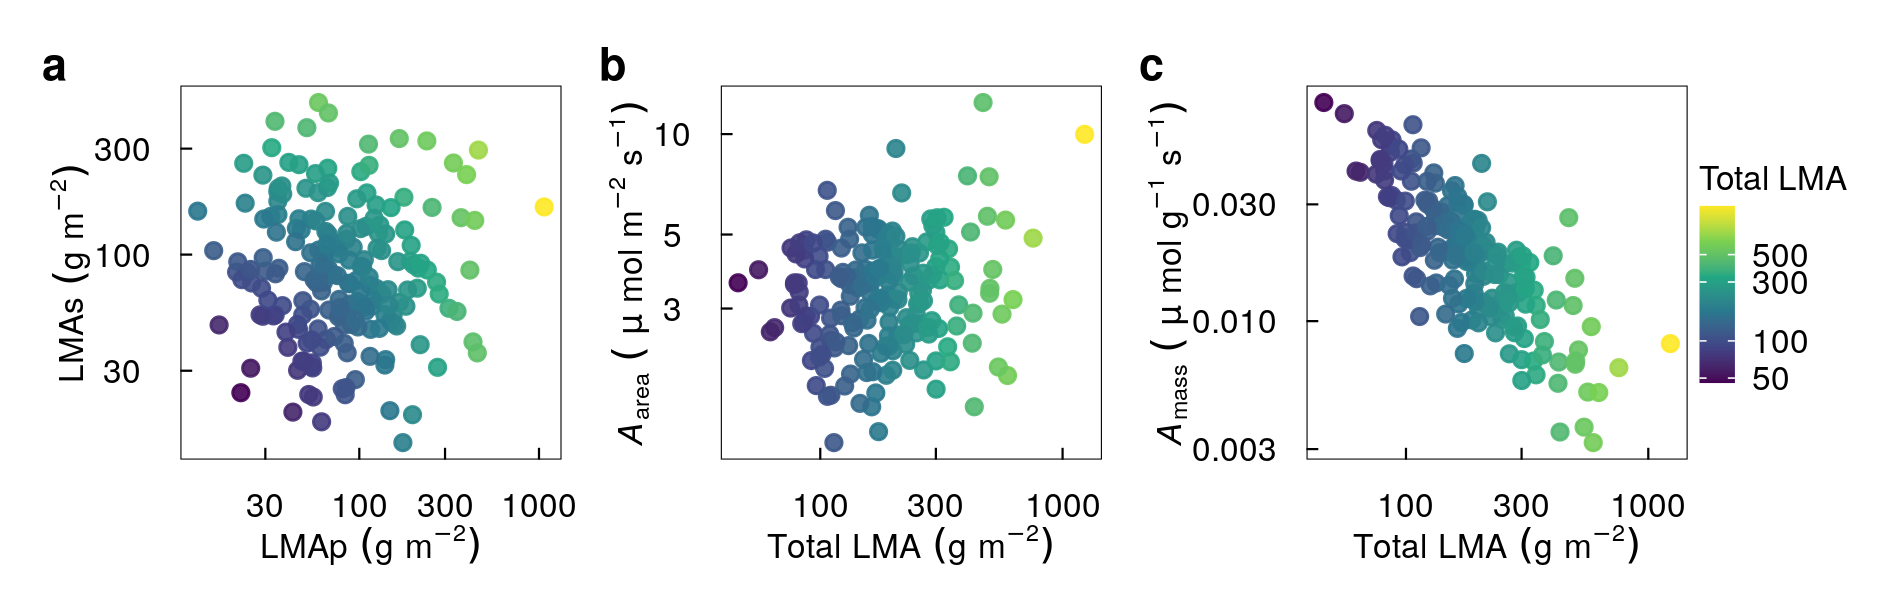
\includegraphics{/Users/mattocci/Dropbox/MS/LMAms/figs/hypo.png}

}

\caption{\label{fig-hypo}Example of a two-dimensional functional space
that can result in either a two- or one-dimensional trait space,
depending on how metabolic traits are normalized. (A) Hypothetical
independent variation in two leaf mass per area (LMA) components:
metabolic leaf mass per area (LMAm, which largely determines per-area
values of photosynthesis, respiration, and nutrient concentrations) and
structural leaf mass per area (LMAs, which determines leaf toughness but
has little effect on metabolic traits). (B) Two-dimensional relationship
between photosynthetic capacity (\emph{A}\textsubscript{max}) per-unit
leaf area and total LMA (equal to LMAm + LMAs). (C) One-dimensional
relationship between \emph{A}\textsubscript{max} per-unit leaf mass and
total LMA. LMAm and LMAs are simulated from a hypothetical scenario of
lognormal distributions with medians of 80 and standard deviations of
exp(0.8) and exp(0.7), and zero covariance. Variation in
\emph{A}\textsubscript{max} values are derived from our analysis of the
GLOPNET database.
\(A_{\mathrm{area} \, i}=1.77 \times \mathrm{LMAm}_i^{0.28}\mathrm{LMAs}^{-0.13}\epsilon_i\),
where \(\epsilon_i\) is log-normally distributed with log-mean with 0,
log-scale parameter with 0.31 (see Methods and Results).}

\end{figure}

\begin{figure}

{\centering 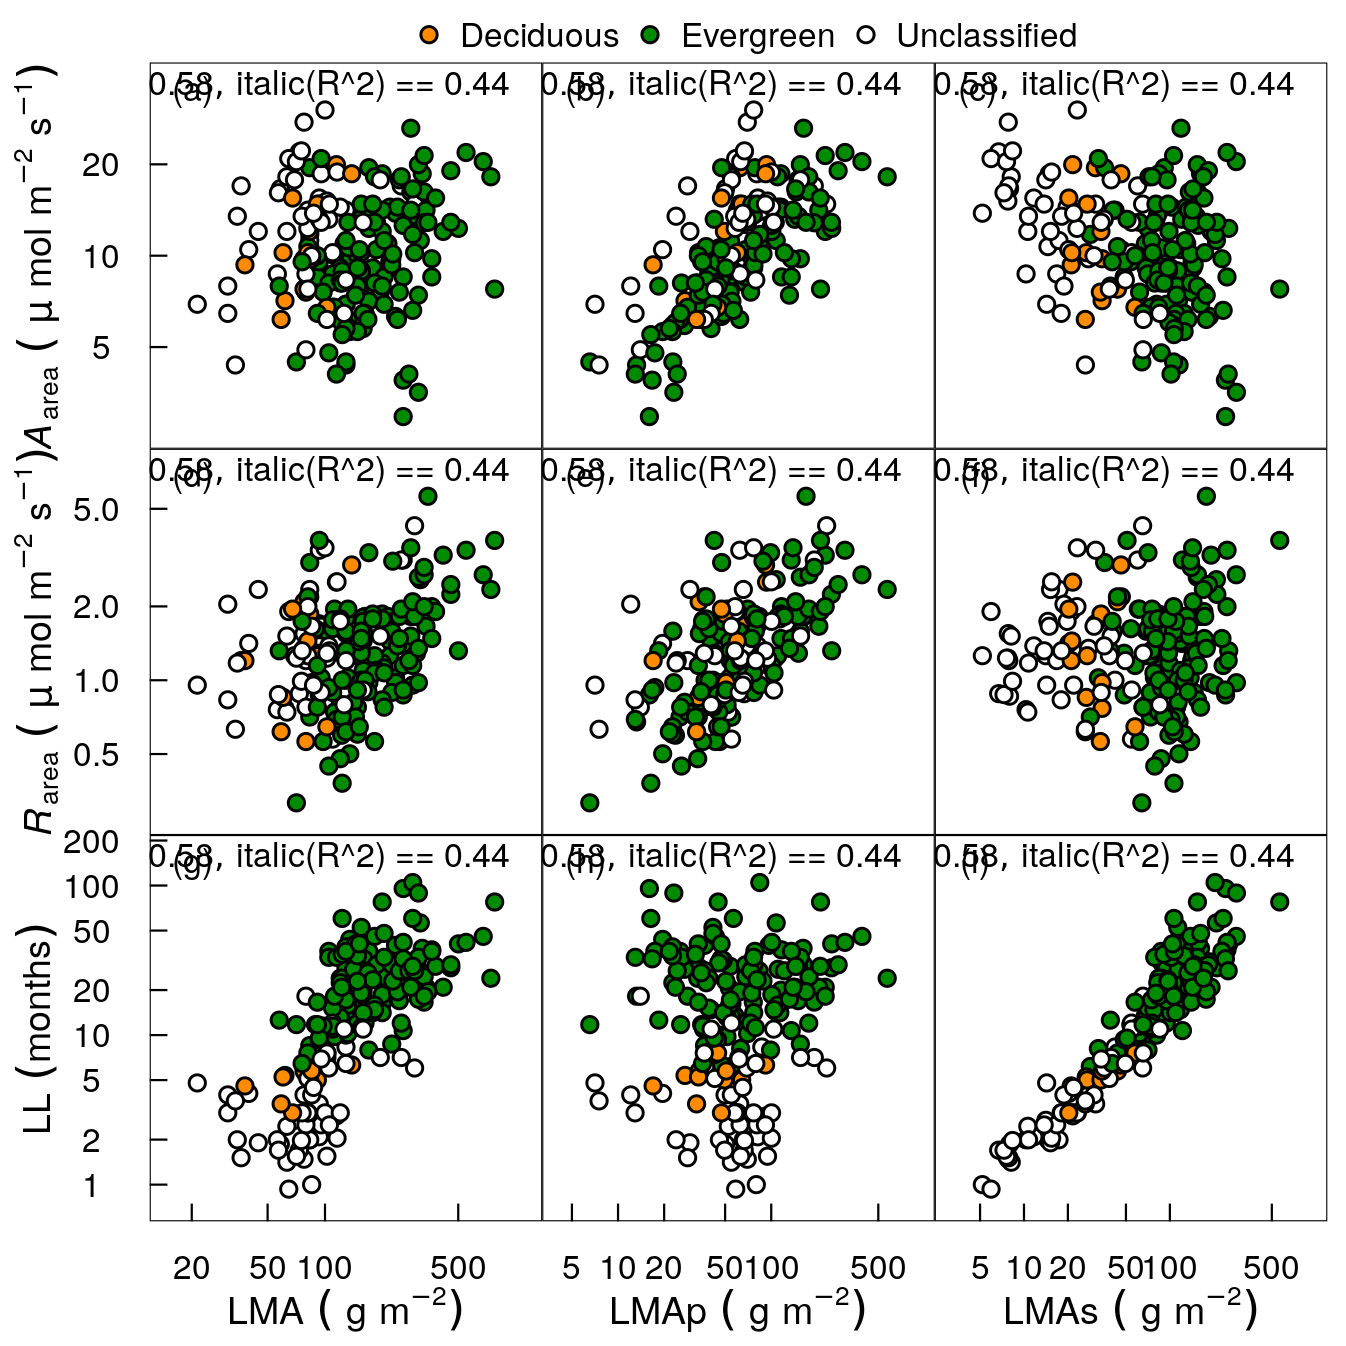
\includegraphics{/Users/mattocci/Dropbox/MS/LMAms/figs/gl_point.png}

}

\caption{\label{fig-gl_point}Observed and estimated leaf-trait
relationships in the global GLOPNET dataset. Estimates are from the best
GLOPNET model (Table 1). Leaf life span (LL), net photosynthetic rate
per unit leaf area (\emph{A}\textsubscript{area}), and dark respiration
rate per unit leaf area (\emph{R}\textsubscript{area}) are plotted
against observed LMA, posterior medians of LMAm and LMAs. Pearson
correlation coefficients (\emph{r}) for LMA (left column) and posterior
medians of Pearson correlation coefficients (\(\bar{r}\)) or partial
correlation coefficients (\(\bar{\rho}\)) for LMAm (middle column) and
LMAs (right column) are shown. Note that LL was modeled by LMAs alone
due to improved model performance with this parameter constraint (Table
1). Therefore, \emph{r} is reported for LL (single predictor variable),
whereas (\(\bar{\rho}\)) is reported for \emph{A}\textsubscript{area}
and \emph{R}\textsubscript{area} (multiple predictor variables).}

\end{figure}

\newpage

\begin{figure}

{\centering 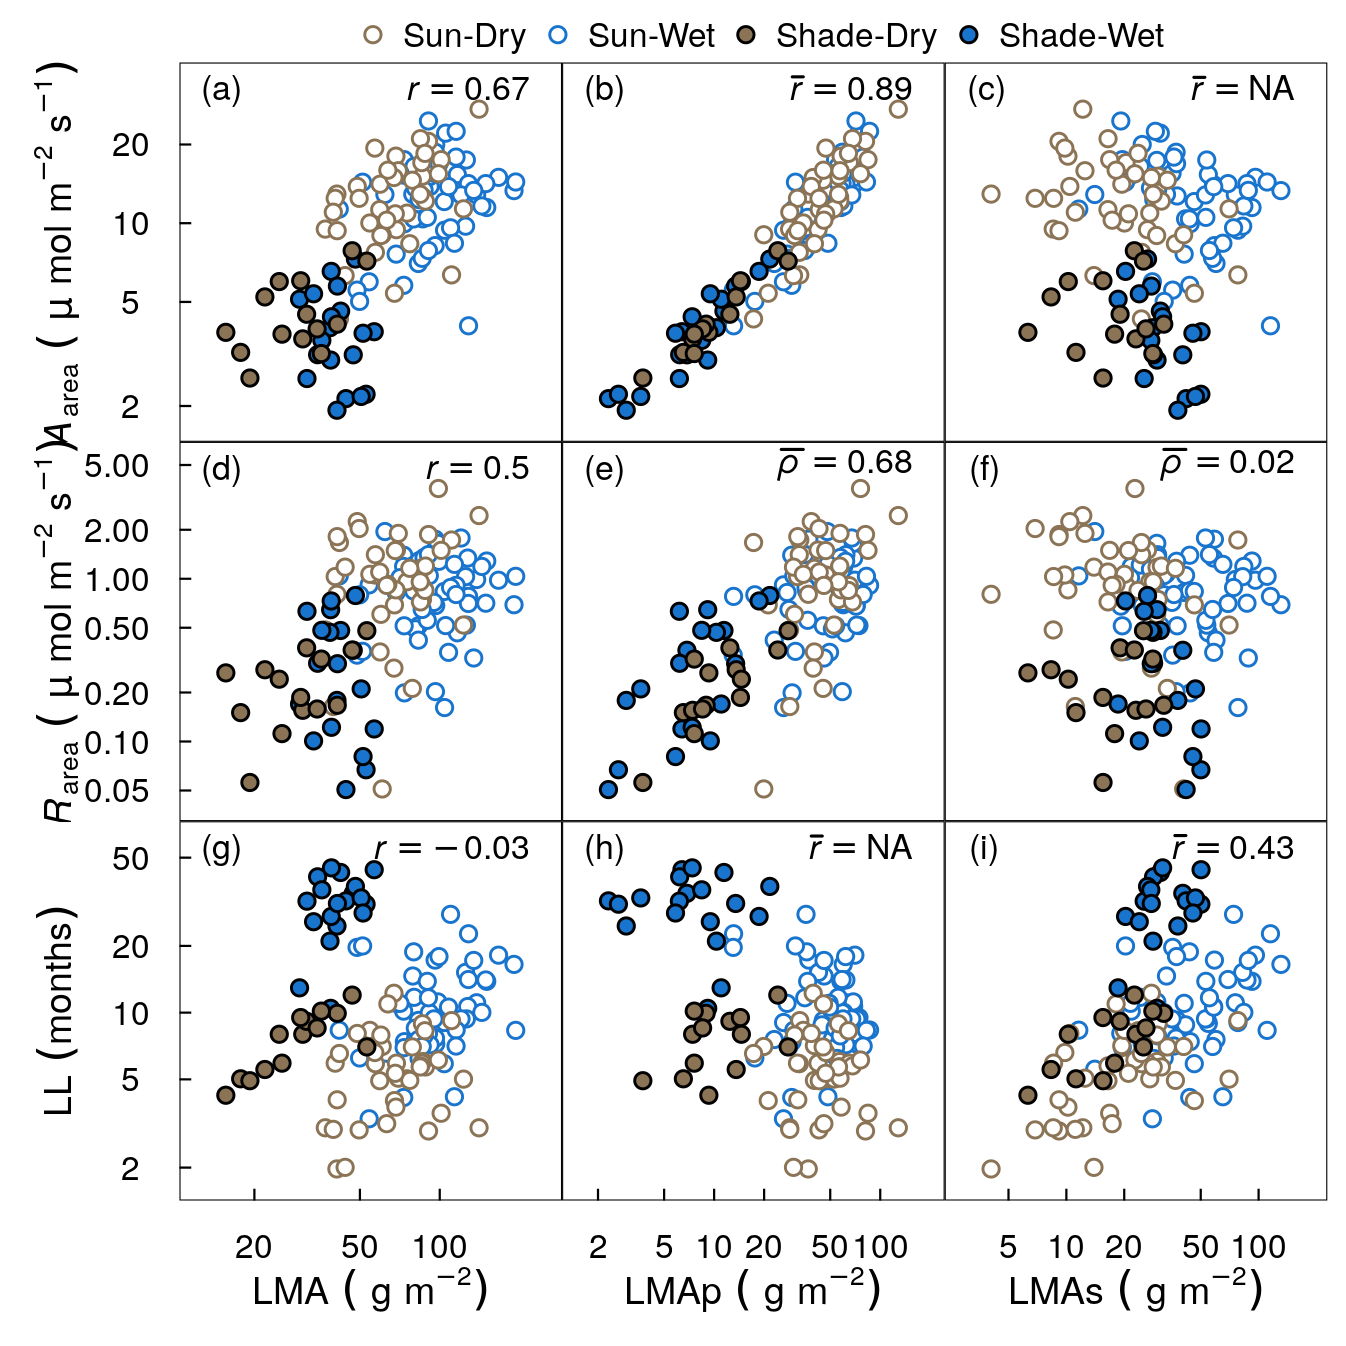
\includegraphics{/Users/mattocci/Dropbox/MS/LMAms/figs/pa_point.png}

}

\caption{\label{fig-pa_point}Observed and estimated leaf-trait
relationships in the Panama dataset. Estimates are from the best Panama
model (Table 1), which included effects of light on LL. Details as for
Fig.~\ref{fig-gl_point}. Results for other LL models are summarized in
Table SX. Note that \emph{A}\textsubscript{area} and LL were modeled by
LMAp and LMAs alone, respectively, due to improved model performance
with these parameter constraints (Table 1). The results shown here
include all leaves in the Panama dataset. The observed separation of LL
between sun and shade leaves is accounted for in the model predictions
Fig.~\ref{fig-ll_point}.}

\end{figure}

\newpage

\begin{figure}

{\centering \includegraphics{/Users/mattocci/Dropbox/MS/LMAms/figs/pa_point_par_ll.png}

}

\caption{\label{fig-ll_point}Relationship between leaf lifespan (LL) and
LMAs in the Panama dataset, afeter accounting for the effects of light
(suv vs.~shade leaves; see Eq. 4b). The dashed line indicates the 1:1
relationship expected for residuals on the log-scale. The posterior
medians of the partial correlation coefficient (\(\bar{\rho}\)) is
shown. The results shown here include all leaves in the Panama dataset.}

\end{figure}

\newpage

\begin{figure}

{\centering \includegraphics{/Users/mattocci/Dropbox/MS/LMAms/figs/vpart_intra.png}

}

\caption{\label{fig-vpart}Variance partitioning on LMA components
between and within leaf habits (evergreen vs.~deciuous) for the GLOPNET
dataset and the Panama dataset, and between and within sites (wet
vs.~dry) and light (sun vs.~shade) for the Panama dataset. To isolate
the effects of intraspecific variation, the Panama results shown here
only include species for which both sun and shade leaves were
available.}

\end{figure}

\newpage

\begin{figure}

{\centering \includegraphics{/Users/mattocci/Dropbox/MS/LMAms/figs/box_de.png}

}

\caption{\label{fig-box_de}Boxplots comparing leaf mass per area (LMA)
and posterior medians of photosynthetic and structural LMA components
(LMAm and LMAs, respectively) across deciduous (Dev) and evergreen (Eve)
leaves in the GLOPNET dataset (a) and in the Panama dataset (b). The
center line in each box indicates the median, upper and lower box edges
indicate the interquartile range, whiskers show 1.5 times the
interquartile range, and points are outliers. Groups sharing the same
letters are not significantly different (P \textgreater{} 0.05;
t-tests). The Panama results only include species for which both sun and
shade leaves were available. Qualitatively similar results were obtained
when all Panama species were included (Fig. S1). Note that the vertical
axis is on a log\textsubscript{10} scale.}

\end{figure}

\newpage

\begin{figure}

{\centering \includegraphics{/Users/mattocci/Dropbox/MS/LMAms/figs/box_pa.png}

}

\caption{\label{fig-box_pa}Boxplots comparing leaf mass per area (LMA)
and posterior medians of metabolic and structural LMA components (LMAm
and LMAs, respectively) across sites (wet and dry) and canopy strata
(sun and shade) in the Panama dataset. These results only include
species for which both sun and shade leaves were available.
Qualitatively similar results were obtained when all Panama species were
included (Fig. S1). Details as for Fig.~\ref{fig-box_de}.}

\end{figure}

\newpage

\begin{figure}

{\centering 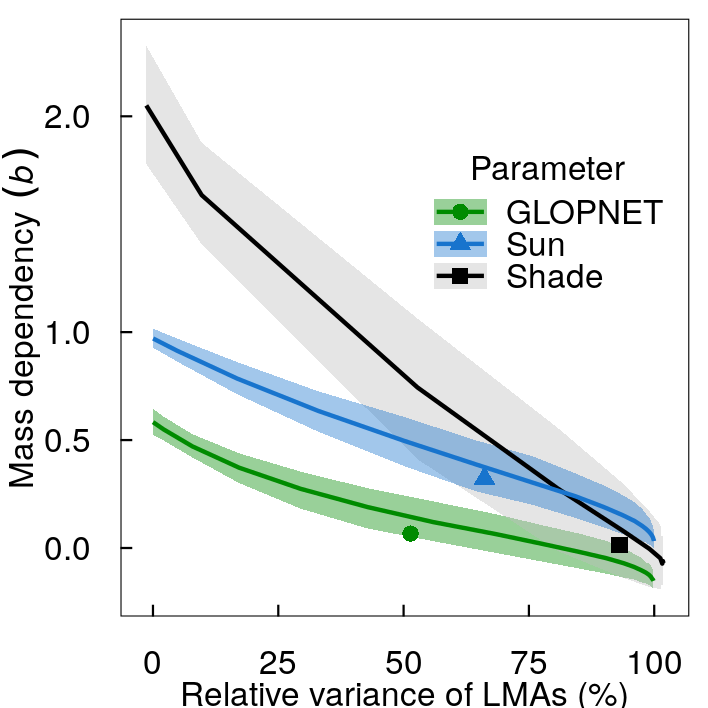
\includegraphics{/Users/mattocci/Dropbox/MS/LMAms/figs/mass_prop_mv.png}

}

\caption{\label{fig-mass_prop}Relationships between mass dependency
(\emph{b} in Eq. 5) and LMAs variance (relative to total LMA variance)
for the global GLPNET datase,t, sun leaves in Panama, and shade leaves
in Panama. Solid lines indicate simulated medians and shaded regions
indicate 95\% CIs. Each point indicates the estimated values from the
empirical data and represents interspecific variation (e.g., across
species within a canopy position in the Panama dataset). The y-axis
values indicates if photosynthetic capacity
(\emph{A}\textsubscript{max}) is is primarily mass-dependent (\emph{b}
\textgreater{} 0.5) or primarily area-dependent (0.5 \textgreater{}
\emph{b} \textgreater{} 0), with \emph{b} near 0 indicating purely
area-dependendence (\protect\hyperlink{ref-Osnas2018}{Osnas et al.,
2018}). If \emph{b} \textgreater{} 1, then \emph{A}\textsubscript{max}
increases exponentially with LMA, which is not consistent with observed
relationships (\protect\hyperlink{ref-Osnas2018}{Osnas et al., 2018}).}

\end{figure}

\newpage

\begin{figure}

{\centering 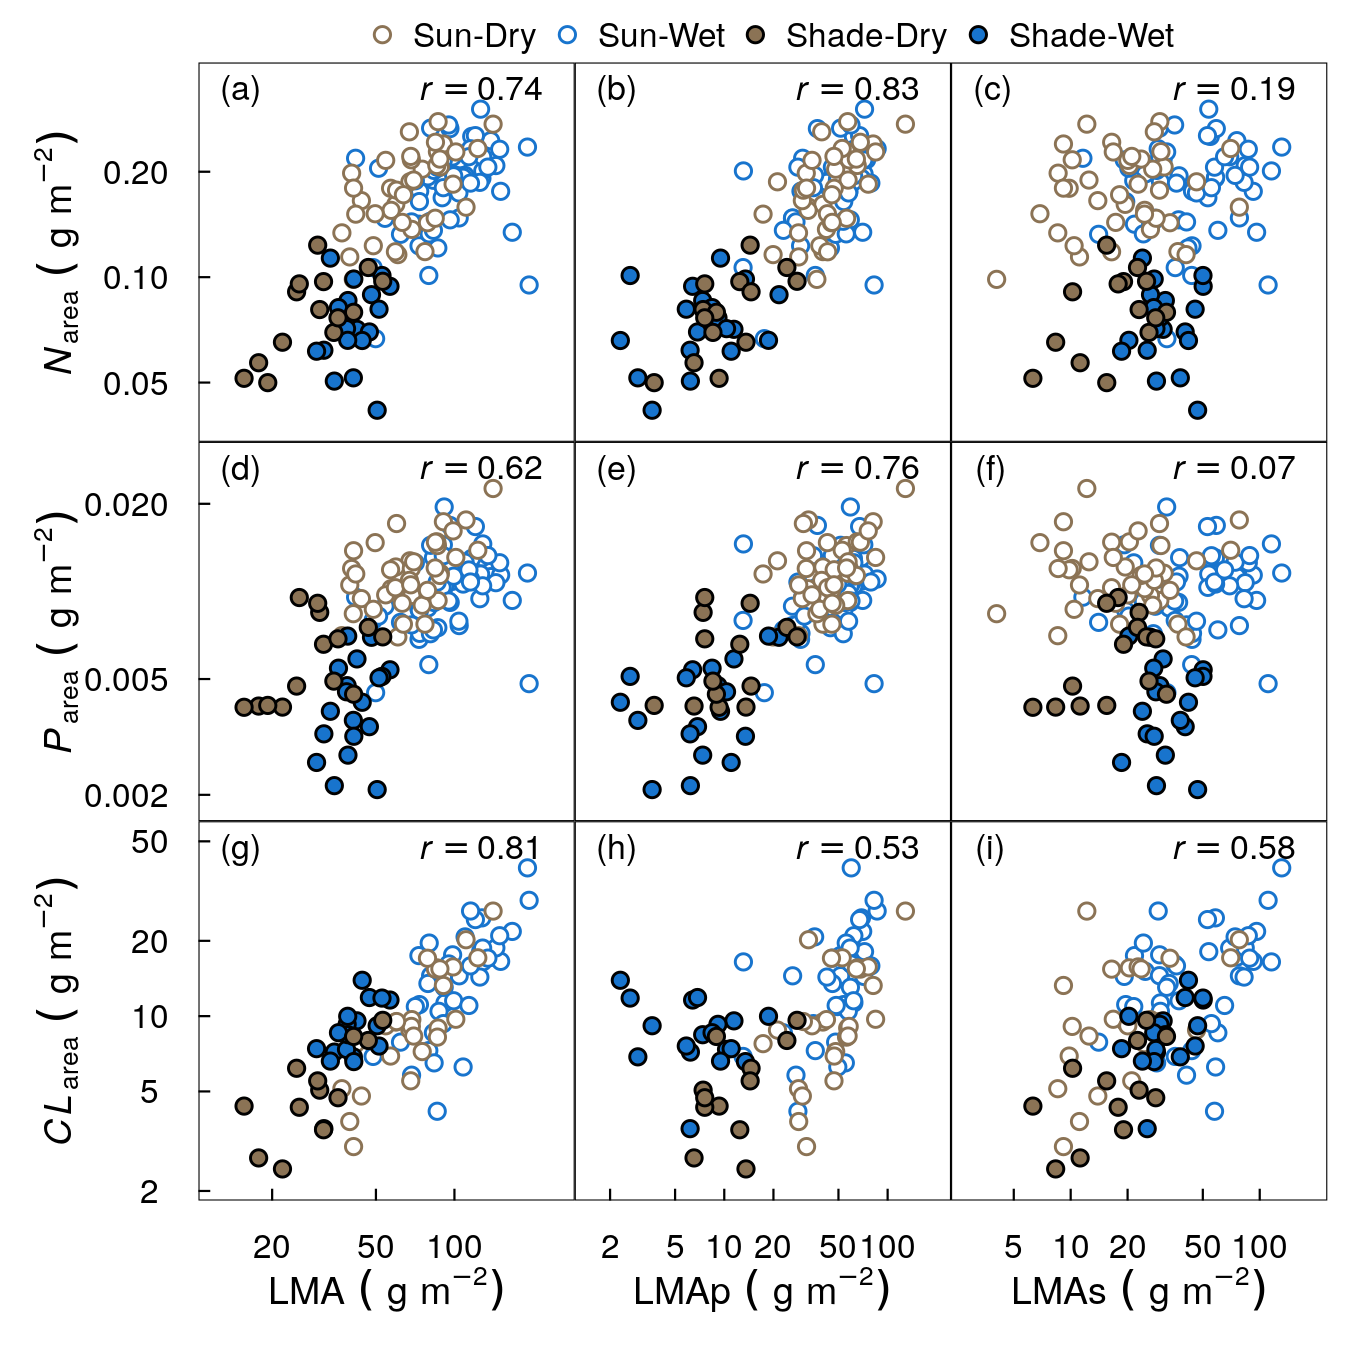
\includegraphics{/Users/mattocci/Dropbox/MS/LMAms/figs/pa_point_npc.png}

}

\caption{\label{fig-pa_npc}Measured traits in the Panama dataset related
to photosynthesis and metabolism (nitrogen and phosphorus per-unit leaf
area; \emph{N}\textsubscript{area} and \emph{P}\textsubscript{area}) are
better correlated with estimates (posterior medians) of the metabolic
LMA component (LMAm) than the strctural component (LMAs), whereas the
opposite patten occurs for a measured structural trait (cellulose
per-unit leaf area; CL\textsubscript{area}).
\emph{N}\textsubscript{area}, \emph{P}\textsubscript{area}, and
CL\textsubscript{area} data were not used to fit the models, and are
presented here as independent support for the model results, and thus
posterior distributions of Pearson correlation coefficients cannot be
estimated for LMAm and LMAs. Pearson correlation coefficients (\emph{r})
are shown for all the panels. Analogous results were obtained for
\emph{N}\textsubscript{area} and \emph{P}\textsubscript{area} for
GLOPNET (Fig. S6). The results shown here include all leaves for which
\emph{N}\textsubscript{area}, \emph{P}\textsubscript{area} and
CL\textsubscript{area} are available.}

\end{figure}



\end{document}
